\chapter{Анализ внутренних силовых факторов}

\section{Задача 1}

\begin{floatingfigure}[r]{0.5\textwidth}
    \centering
    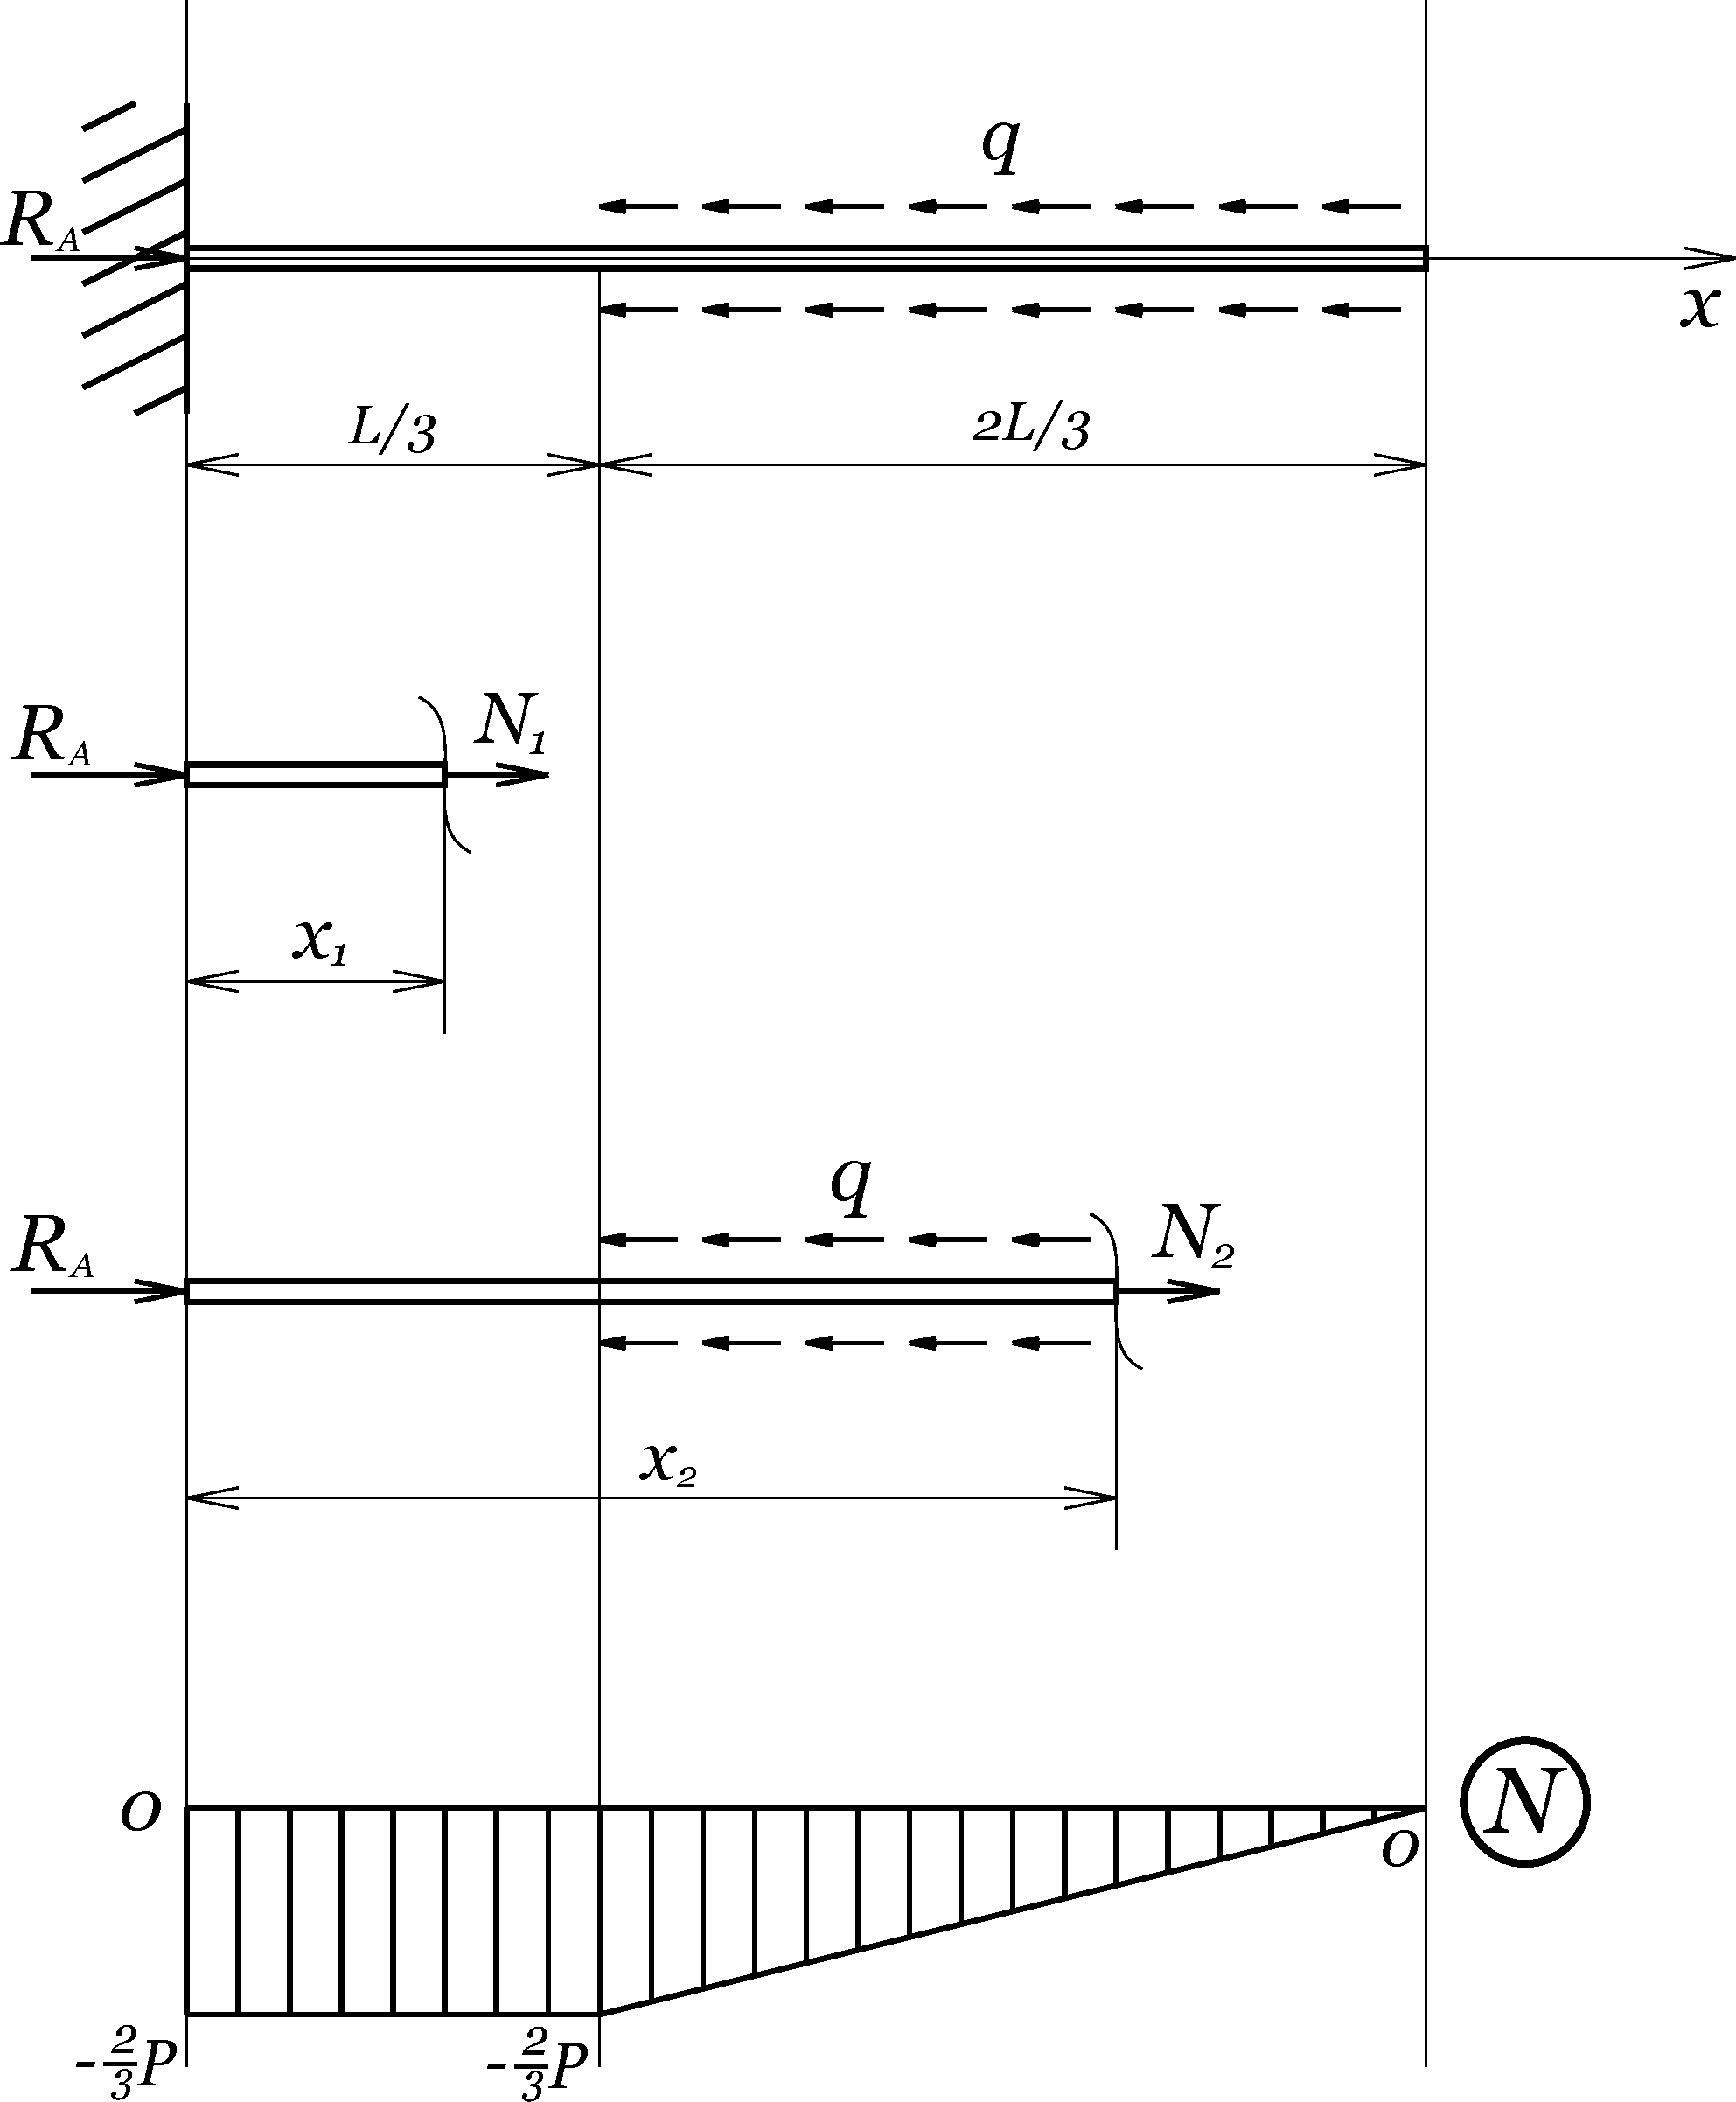
\includegraphics[width=0.5\textwidth]{epura1.pdf}
    \caption{Эпюра продольных сил, $P = qL$.}
    \label{fig:chap1-epura1}
\end{floatingfigure}

$\sum P_x = R_A - q \cdot \frac{2L}{3} = 0$,
откуда
\[
    R_A = \frac{2}{3} P.
\]

Участок 1 $ \left(0 \le x < \frac{L}{3}\right)$

$\sum P_{x} = R_A + N_1 = 0$,
откуда
\[
    N_1 = -\frac{2}{3} P.
\]

Участок 2 $ \left(\frac{L}{3} \le x < L\right)$

$\sum P_{x} = R_A - q \left(x - \frac{L}{3}\right) + N_2= 0$,
откуда
\[
    N_2 = qx - P.
\]

При $x = \frac{L}{3}$: $N_2 = -\frac{2}{3} P$.

При $x = L$: $N_2 = 0$.

\newpage


\section{Задача 2}

\begin{floatingfigure}[r]{0.5\textwidth}
    \centering
    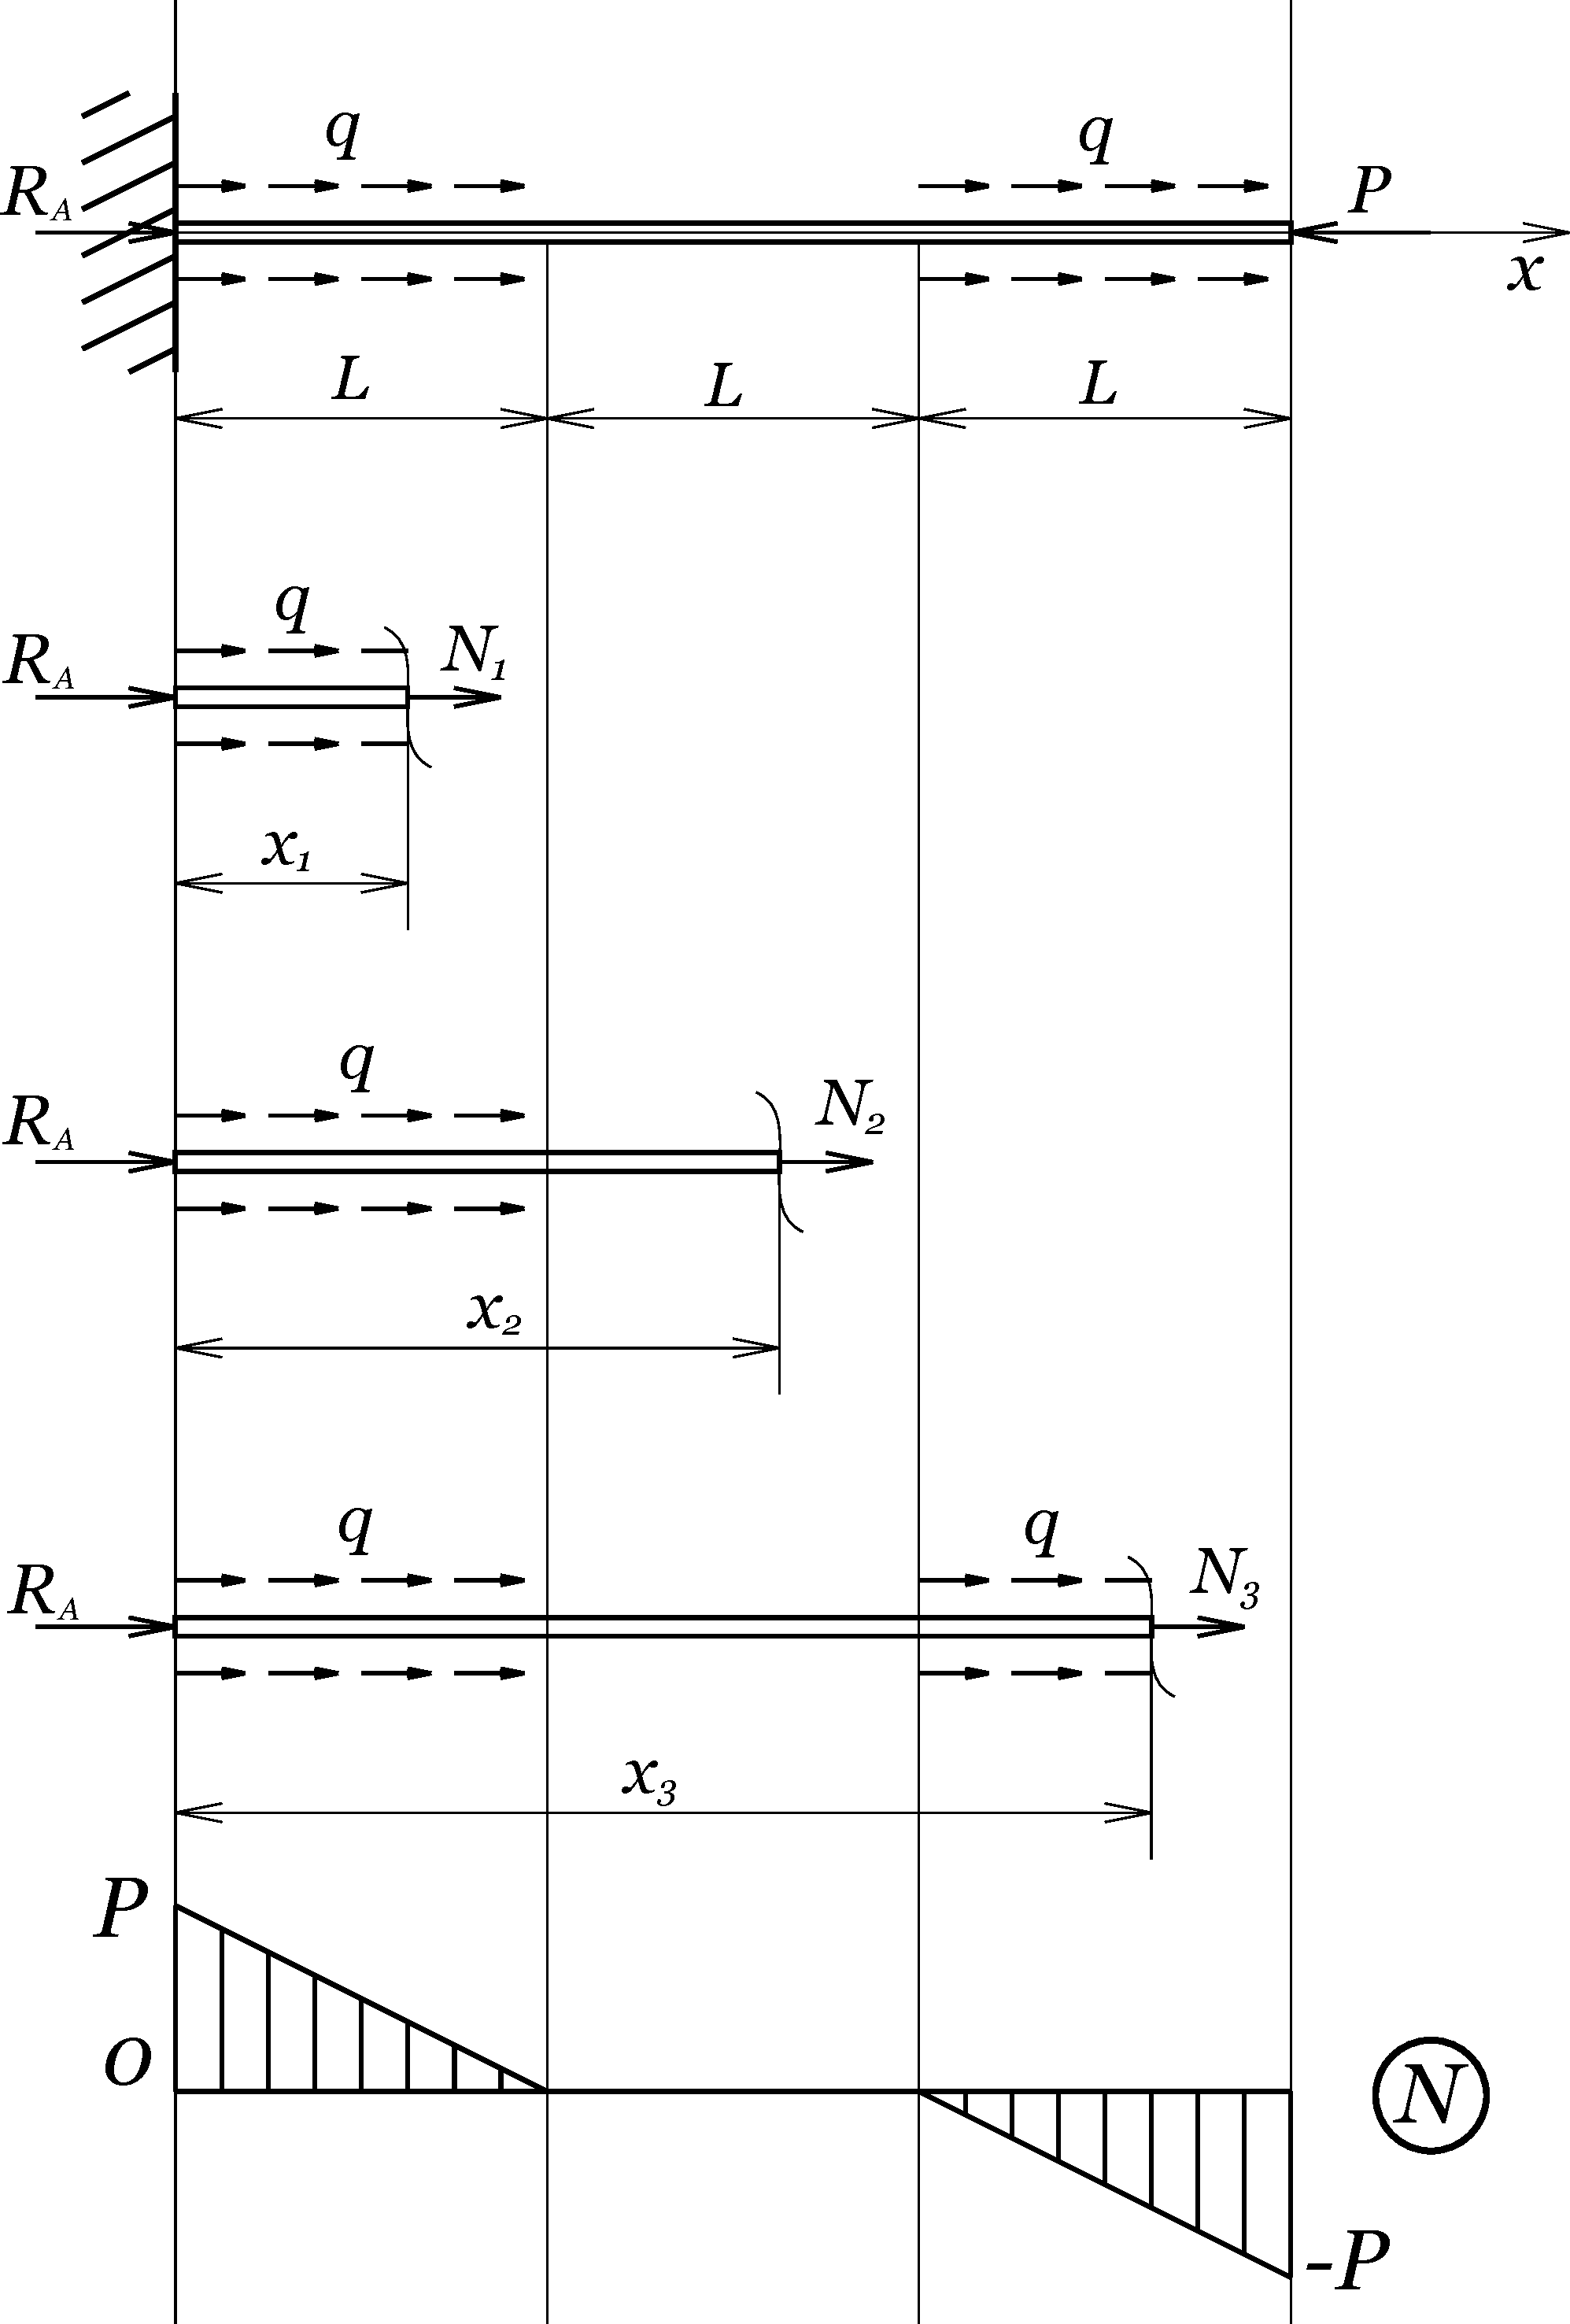
\includegraphics[width=0.5\textwidth]{epura2.pdf}
    \caption{Эпюра продольных сил, $P = qL$.}
    \label{fig:chap1-epura2}
\end{floatingfigure}

$\sum P_x = R_A + qL + qL - P = 0$,
откуда
\[
    R_A = -P.
\]

Участок 1 $\left(0 \le x < L\right)$

$\sum P_{x} = R_A + qx + N_1= 0$,
откуда
\[
    N_1 = -qx + P.
\]

При $x = 0$: $N_1 = P$.

При $x = L$: $N_1 = 0$.

Участок 2 $\left(L \le x < 2L\right)$

$\sum P_{x} = R_A + qL + N_2= 0$,
откуда
\[
    N_2 = 0.
\]

Участок 3 $\left(2L \le x < 3L\right)$

$\sum P_{x} = R_A + qL + q (x - 2L) + N_3 = 0$,
откуда
\[
    N_3 = -qx + 2P.
\]

При $x = 2L$: $N_3 = 0$.

При $x = 3L$: $N_3 = -P$.

\newpage


\section{Задача 3}

\begin{floatingfigure}[r]{0.5\textwidth}
    \centering
    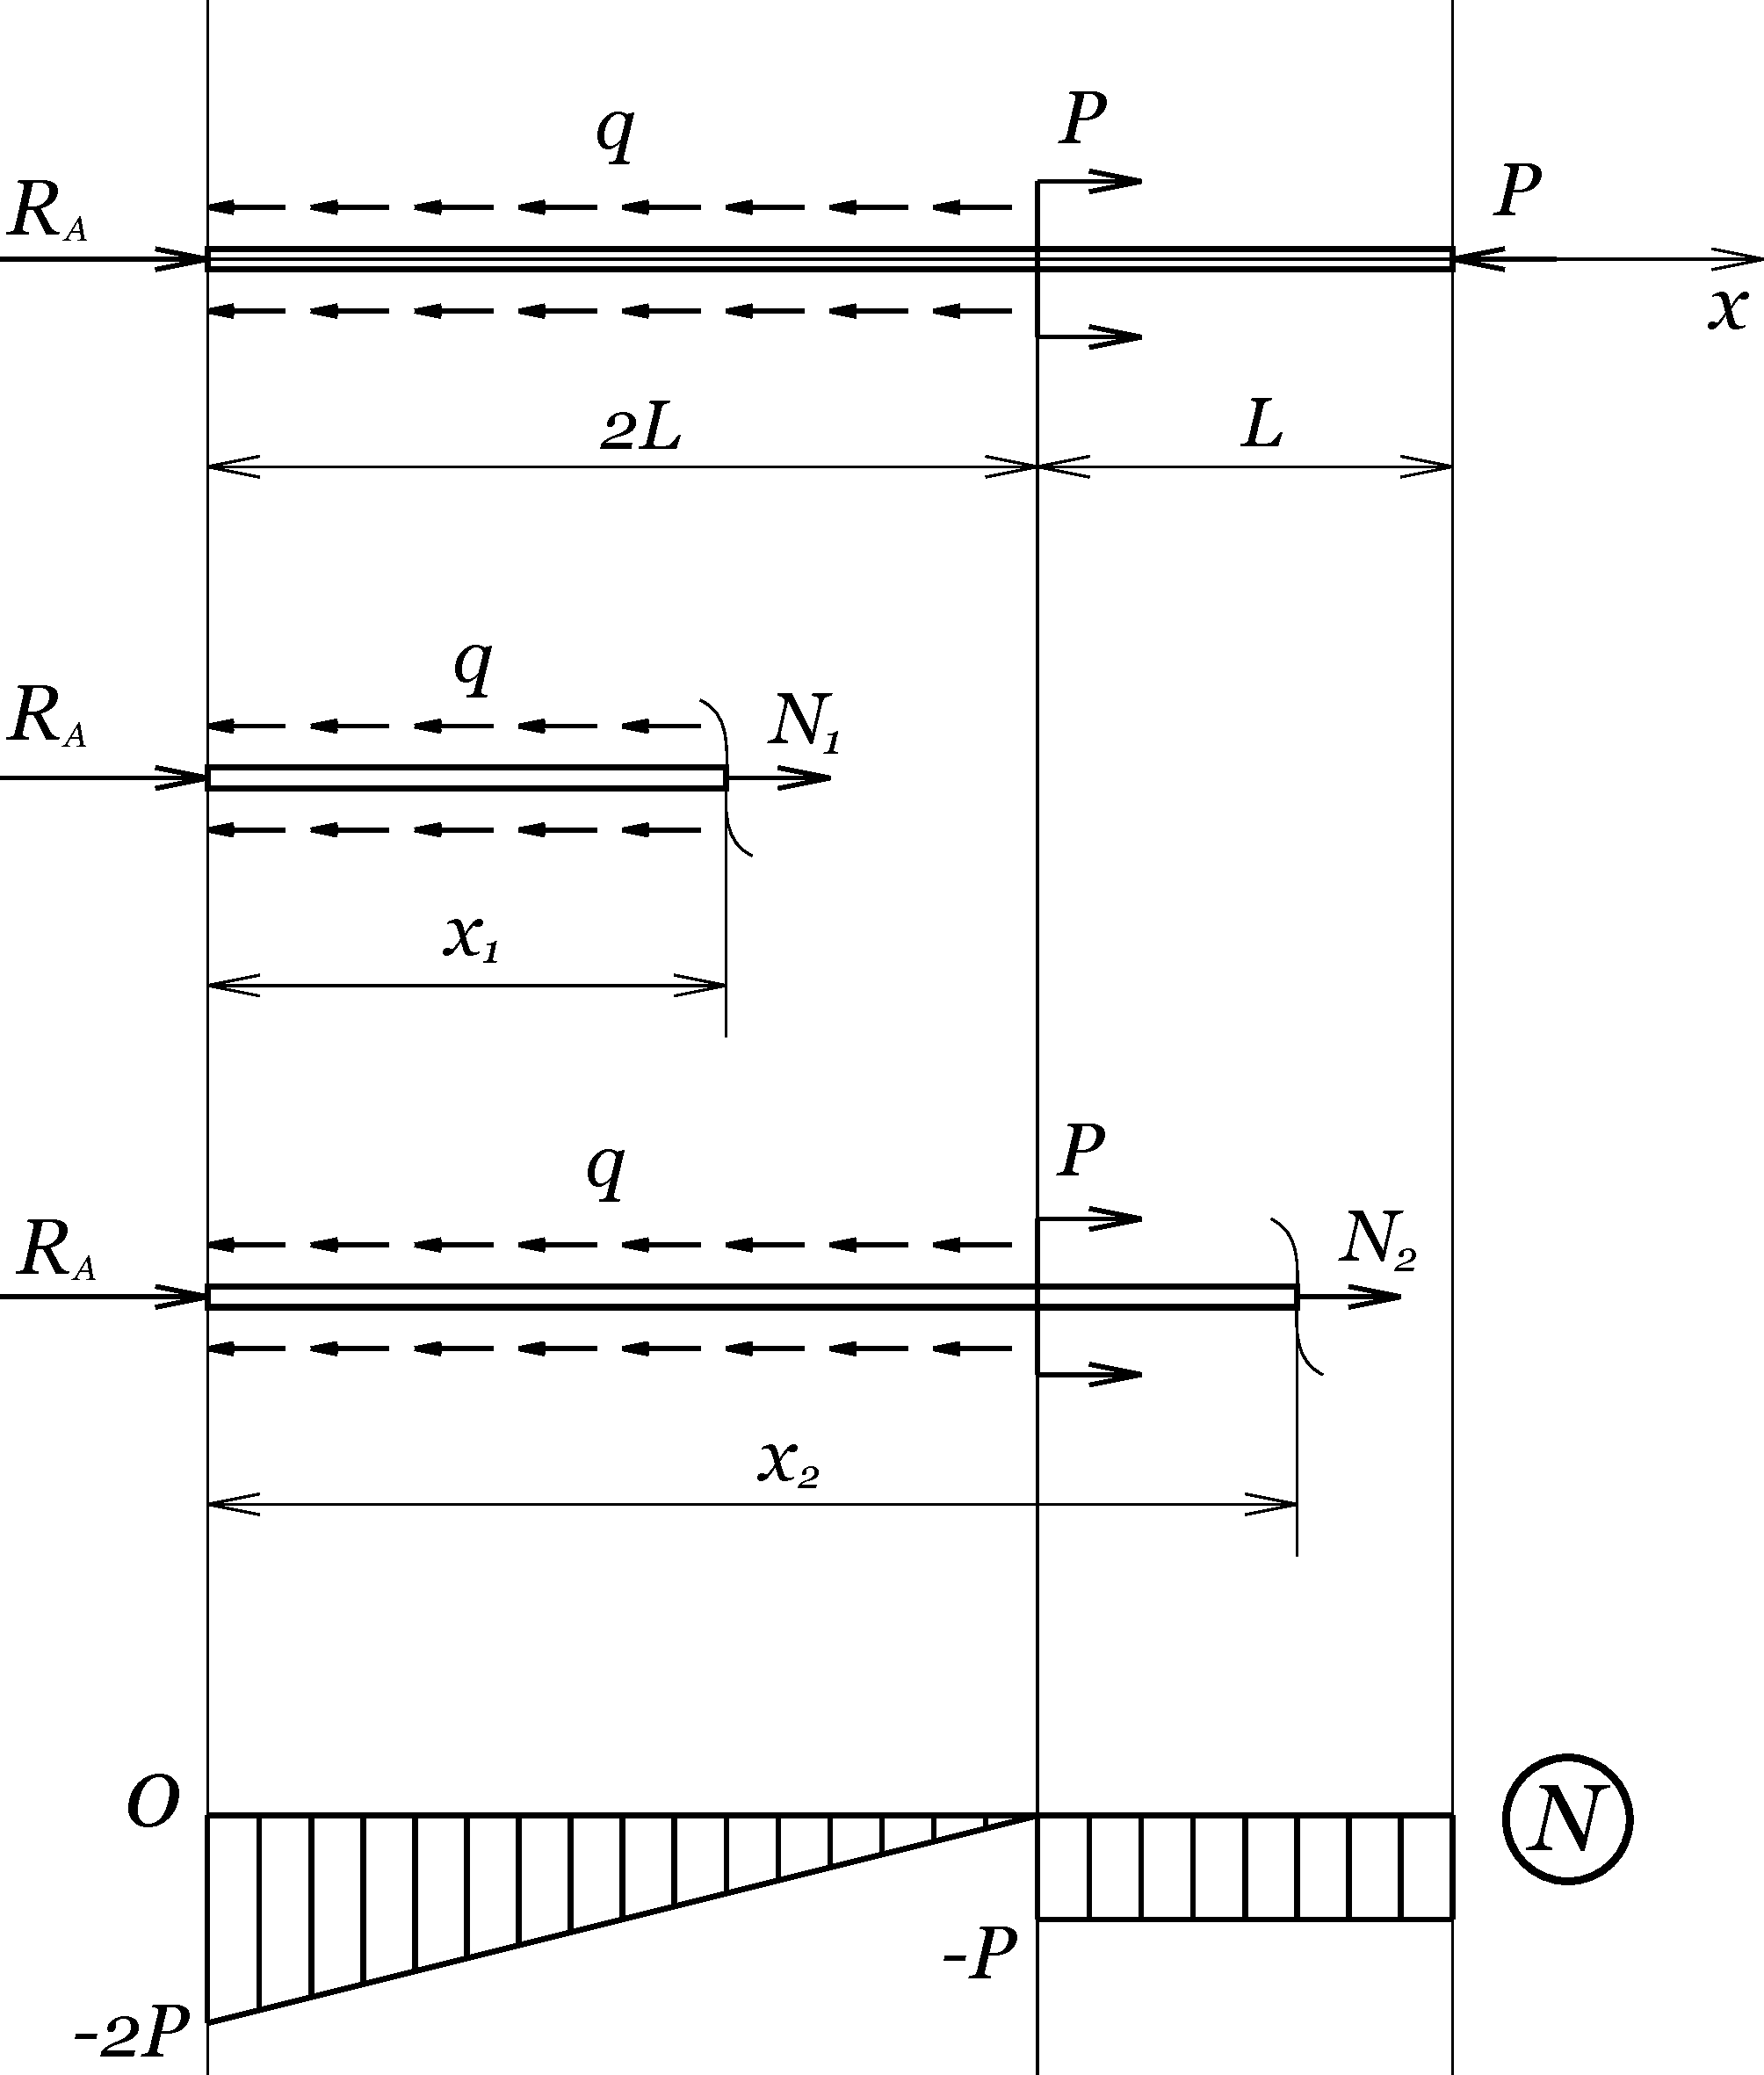
\includegraphics[width=0.5\textwidth]{epura3.pdf}
    \caption{Эпюра продольных сил, $P = qL$.}
    \label{fig:chap1-epura3}
\end{floatingfigure}

$\sum P_x = 2P - q \cdot \left(2L\right) + P - P = 0$

Участок 1 $\left(0 \le x < 2L\right)$

$P_x = 2P - qx + N_1 = 0$,
откуда
\[
    N_1 = qx - 2P.
\]

При $x = 0$: $N_1 = -2 P$.

При $x = 2L$: $N_1 = 0$.

Участок 2 $\left(2L \le x_2 < 3L\right)$

$\sum P_x = 2P - q \cdot \left(2L\right) + P + N_2 = 0$,
откуда
\[
    N_2 = -P.
\]

\newpage


\section{Задача 4}

\begin{floatingfigure}[r]{0.5\textwidth}
    \centering
    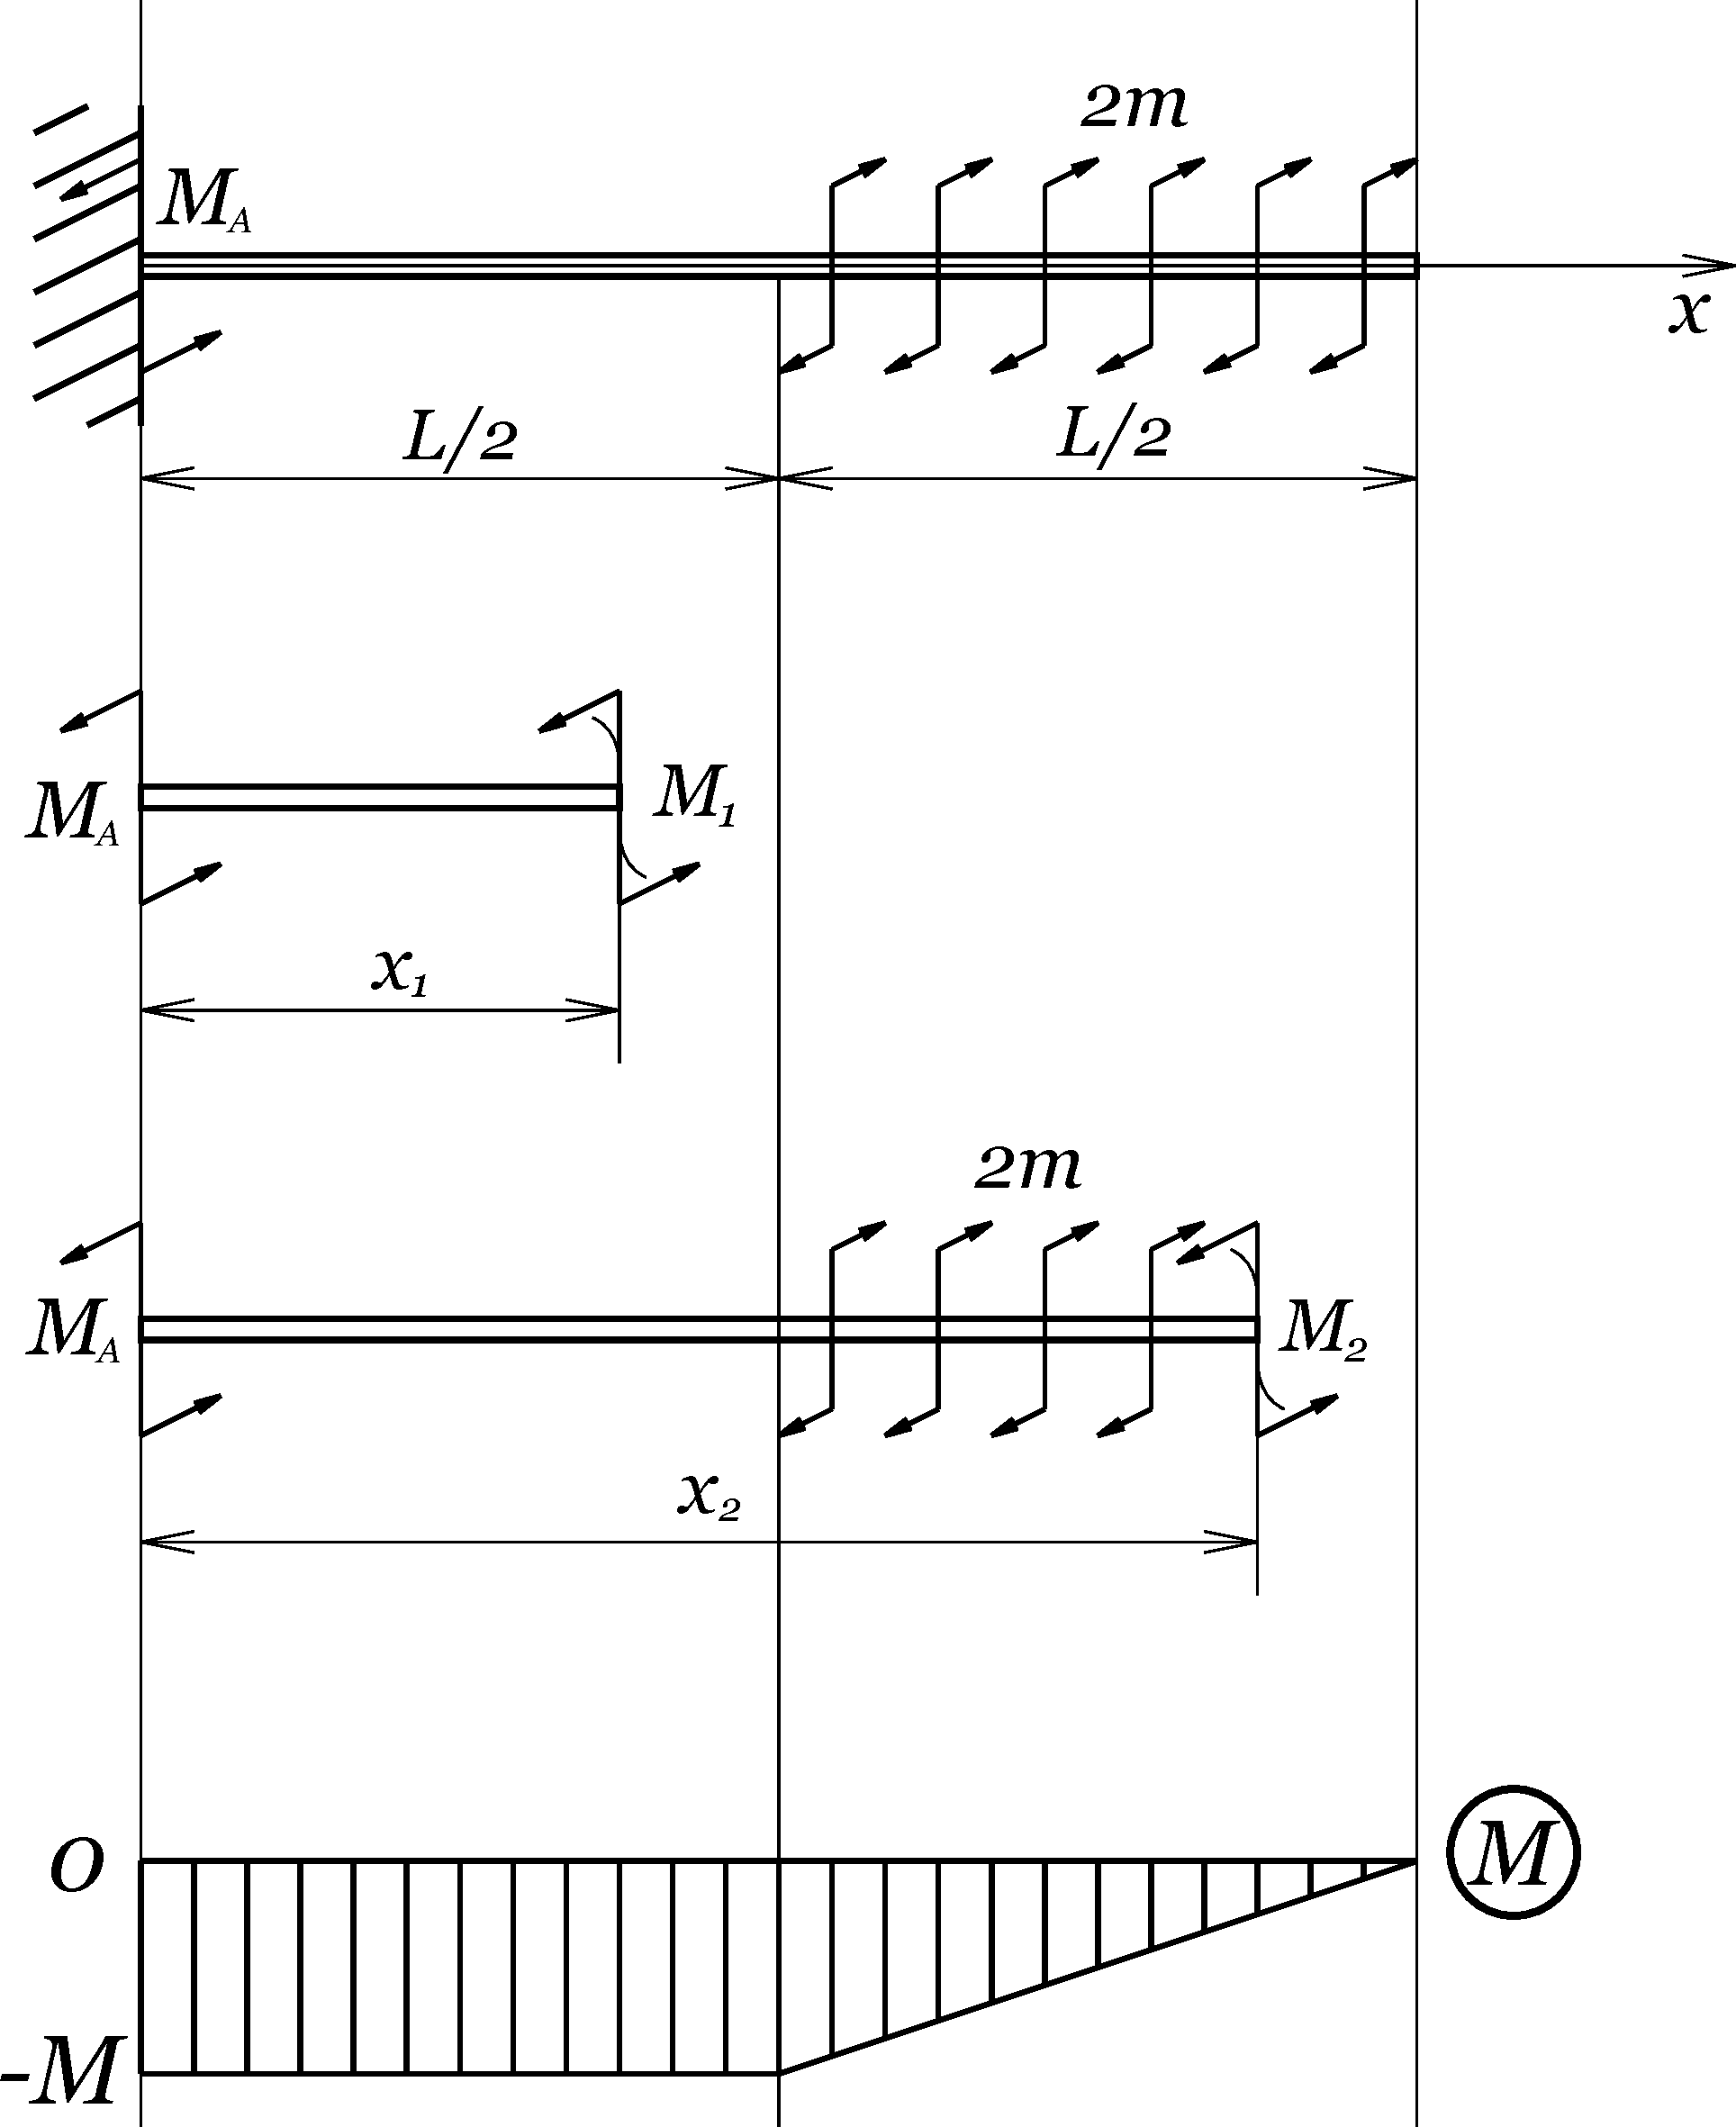
\includegraphics[width=0.5\textwidth]{epura4.pdf}
    \caption{Эпюра моментов, $M = mL$.}
    \label{fig:chap1-epura4}
\end{floatingfigure}

$\sum M_x = M_A - \left(2m\right) \cdot \frac{L}{2} = 0$,
откуда
\[
    M_A = M.
\]

Участок 1 $\left(0 \le x < \frac{L}{2}\right)$

$\sum M_x = M_A + M_1 = 0$,
откуда
\[
    M_1 = -M.
\]

Участок 2 $ \left(\frac{L}{2} \le x < L\right)$

$\sum M_x = M_A + M_2 - 2m \cdot \left(x - \frac{L}{2}\right) = 0$,
откуда
\[
    M_2 = 2mx - 2M.
\]

При $x = \frac{L}{2}$: $M_2 = -M$.

При $x = L$: $M_2 = 0$.

\newpage


\section{Задача 5}

\begin{floatingfigure}[r]{0.5\textwidth}
    \centering
    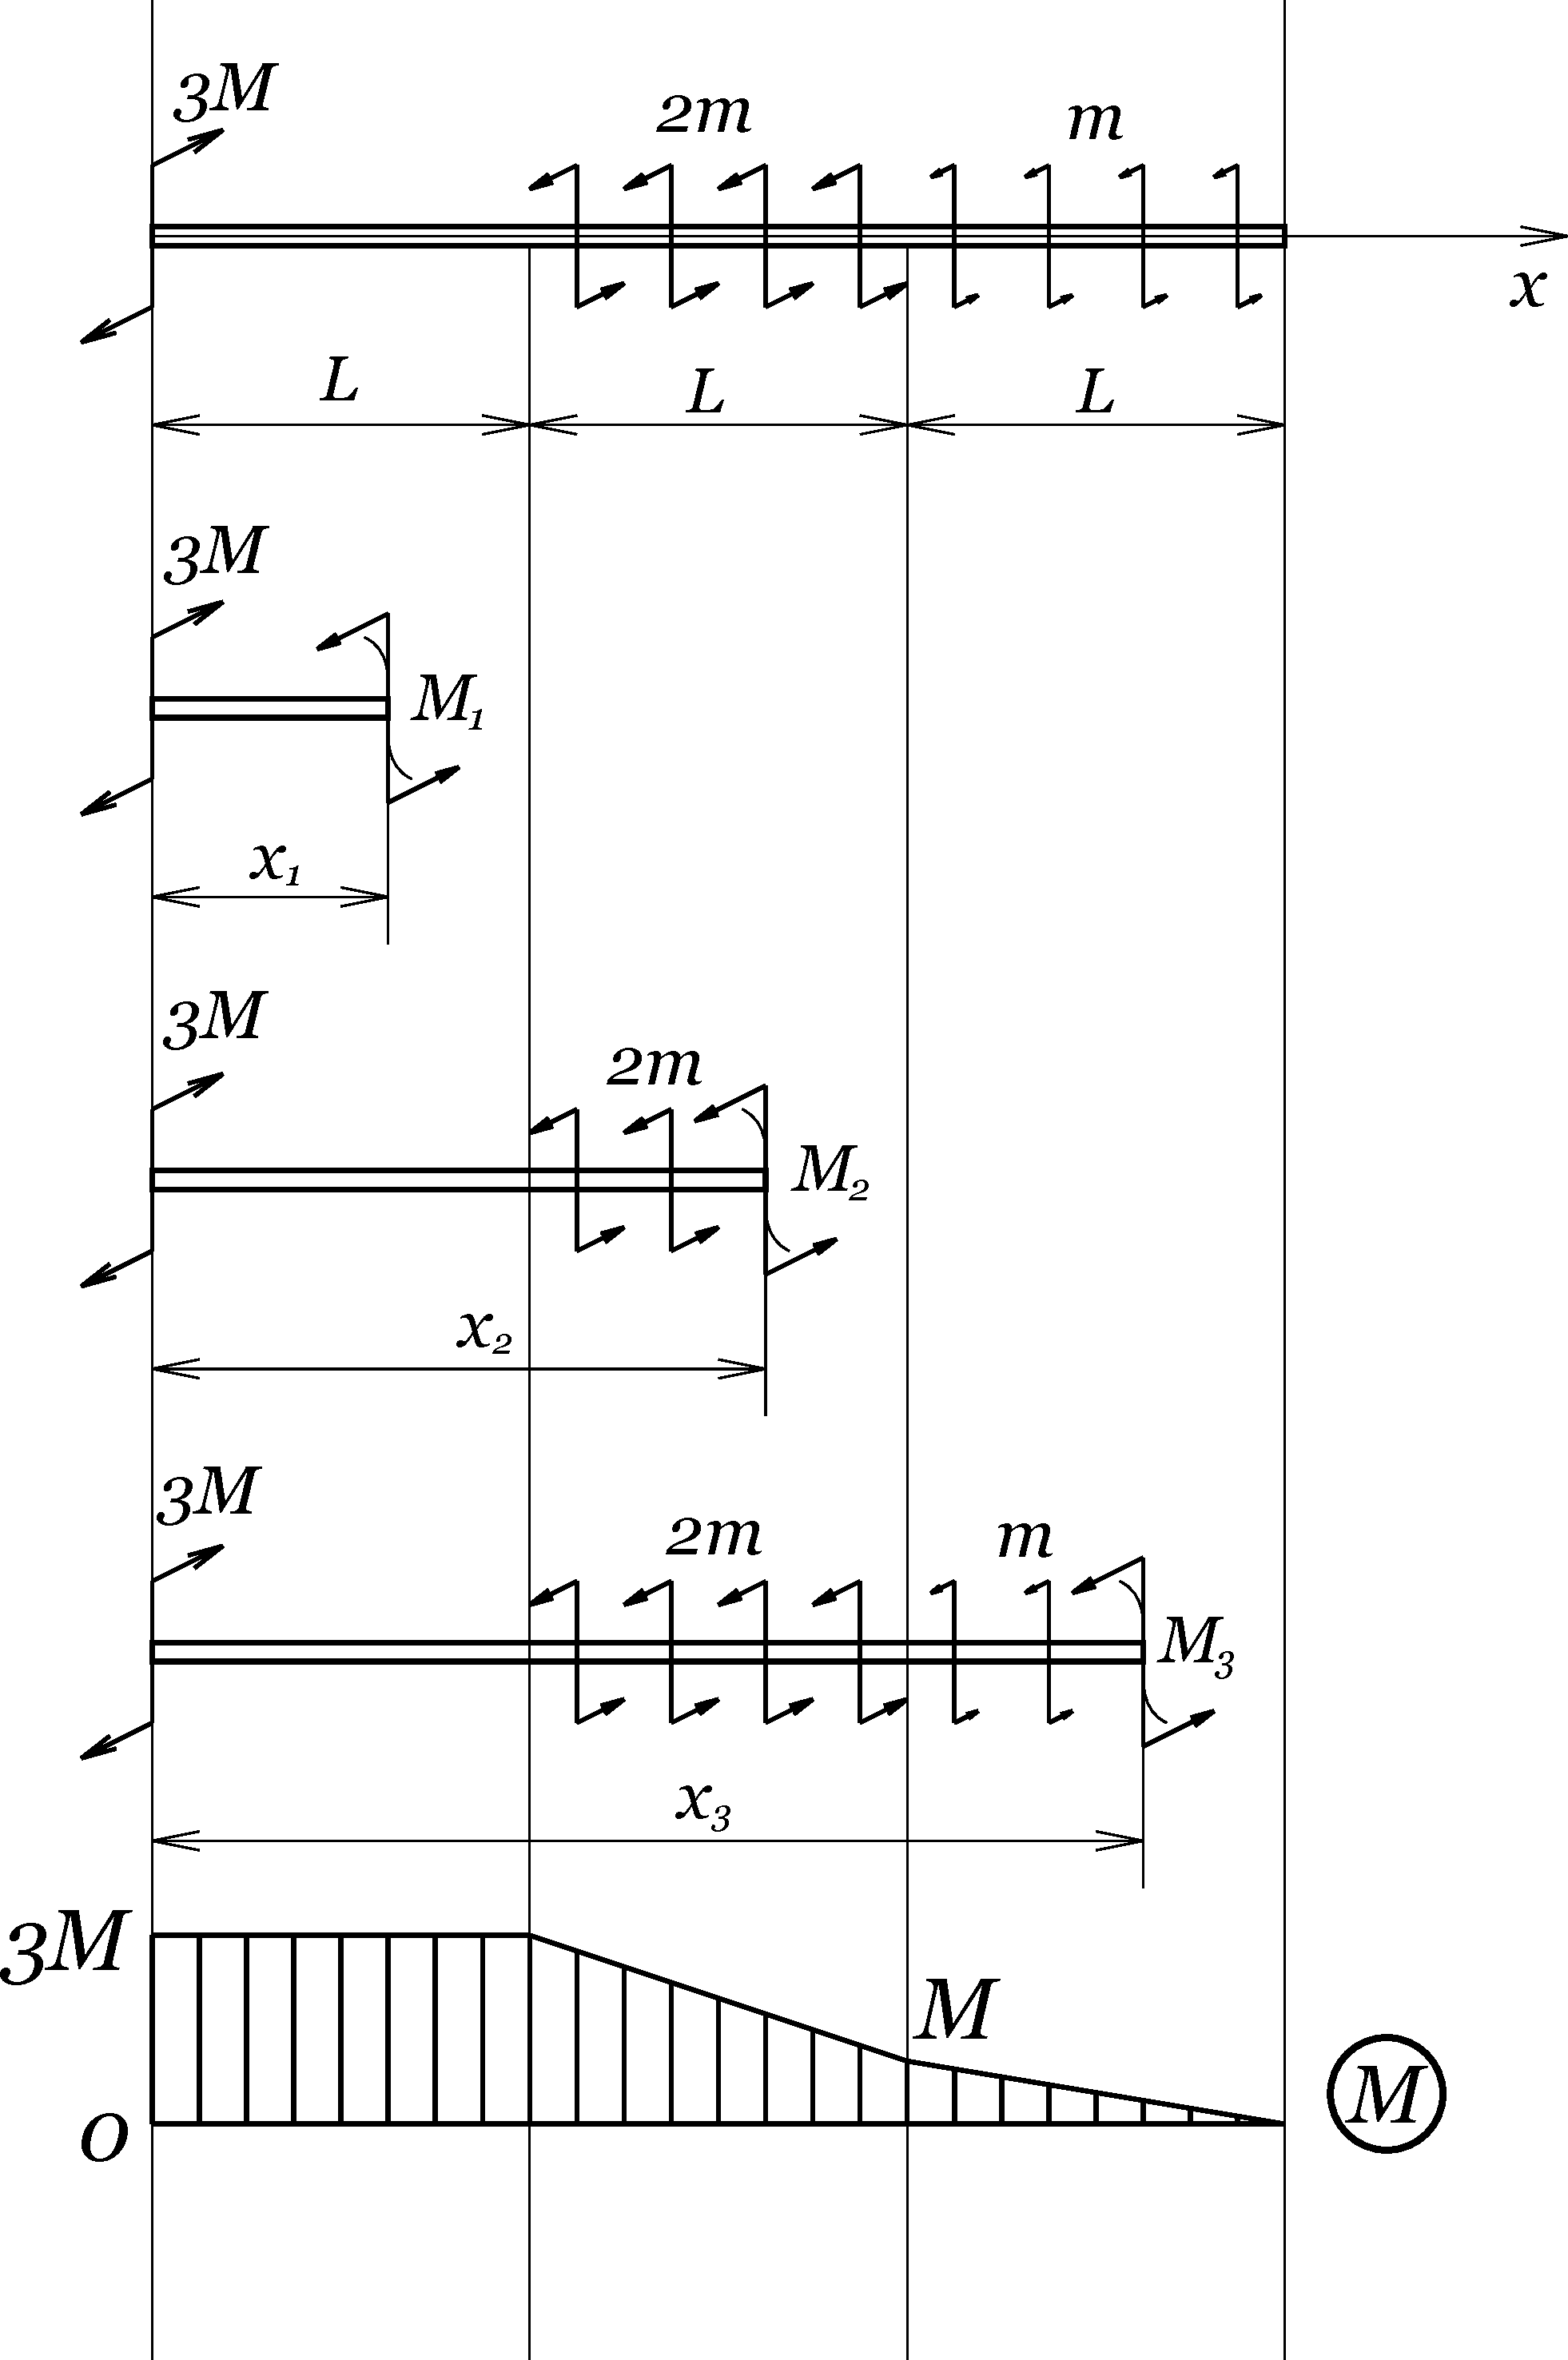
\includegraphics[width=0.5\textwidth]{epura5.pdf}
    \caption{Эпюра моментов, $M = mL$.}
    \label{fig:chap1-epura5}
\end{floatingfigure}

$\sum M_x = -3M + 2mL + mL = 0$.

Участок 1 $\left(0 \le x < L\right)$

$\sum M_x = -3M + M_1 = 0$,
откуда
\[
    M_1 = 3M.
\]

Участок 2 $\left(L \le x < 2L\right) $

$\sum M_x = -3M + 2m \cdot \left(x- L\right) + M_2 =  0$,
откуда
\[
    M_2 = -2mx + 5M.
\]

При $x = L$: $M_2 = 3M$.

При $x = 2L$: $M_2 = M$.

Участок 3 $\left(2L \le x < 3L\right)$

$\sum M_x = -3M + 2mL + m \cdot \left(x- 2L\right) + M_3 = 0$,
откуда
\[
    M_3 = -mx + 3M.
\]

При $x = 2L$: $M_3 = M$.

При $x = 3L$: $M_3 = 0$.

\newpage


\section{Задача 6}

\begin{floatingfigure}[r]{0.5\textwidth}
    \centering
    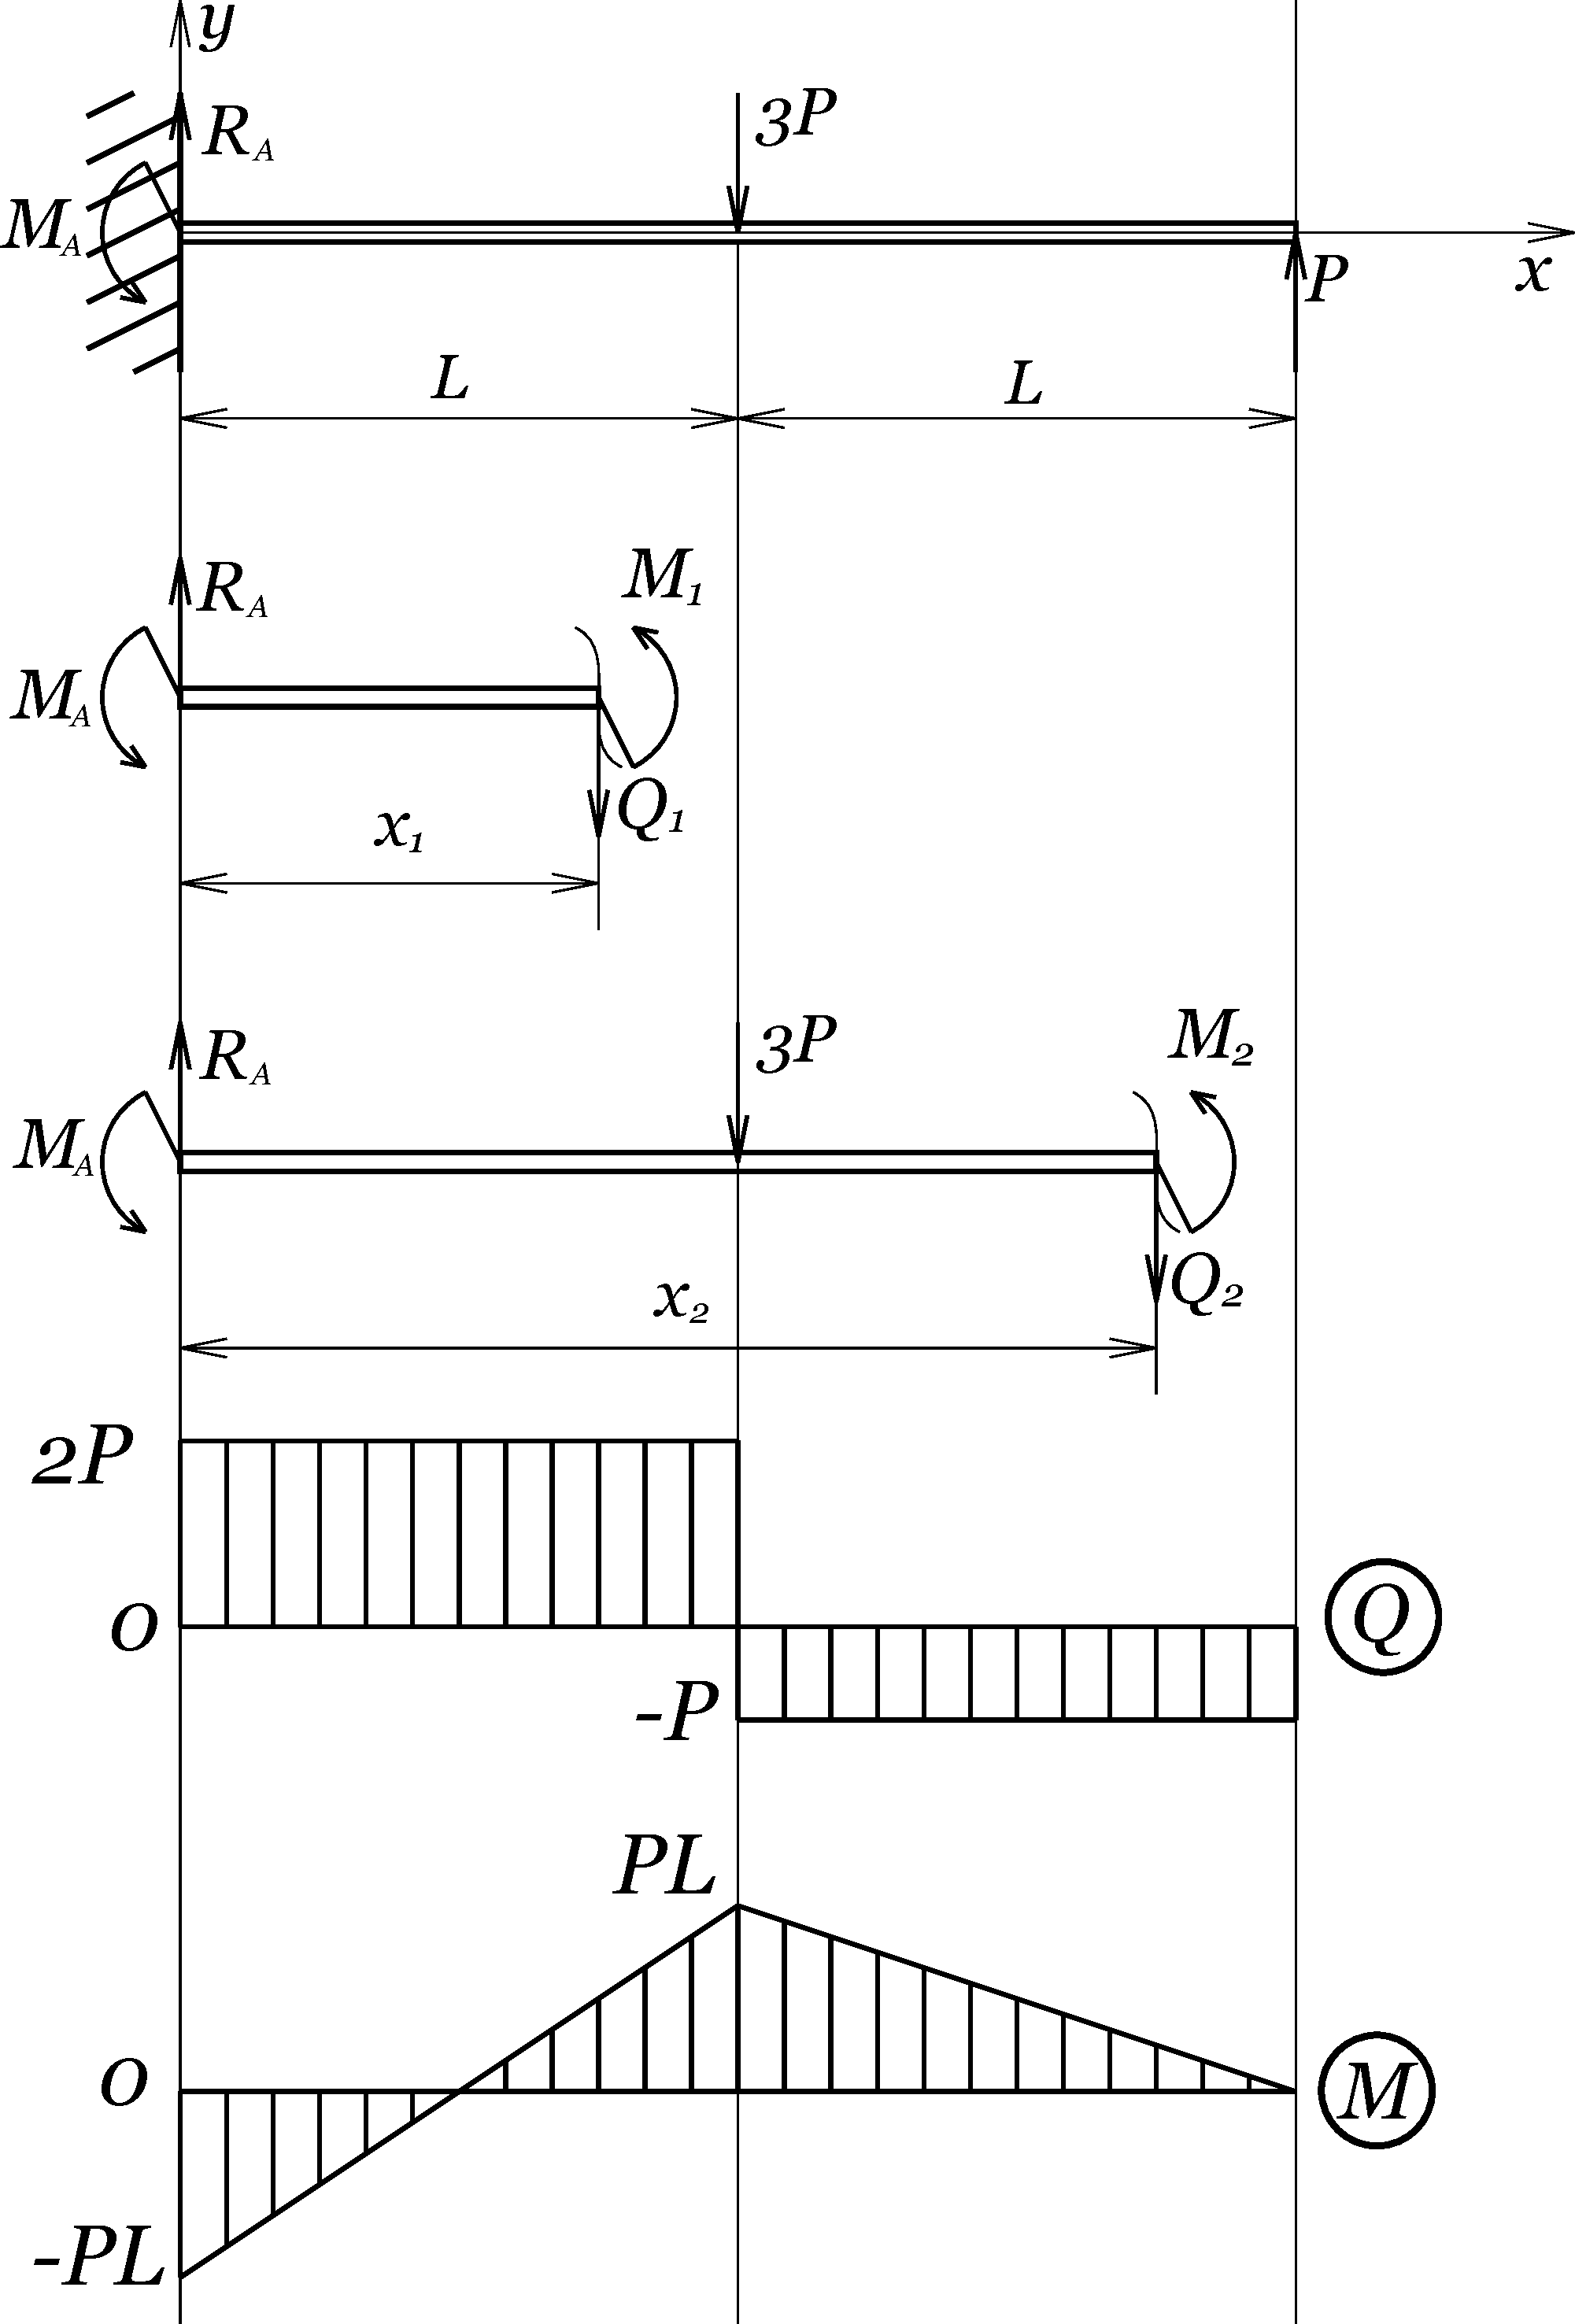
\includegraphics[width=0.5\textwidth]{epura6.pdf}
    \caption{Эпюра поперечных сил и моментов.}
    \label{fig:chap1-epura6}
\end{floatingfigure}

$\sum M_x = M_A - 3P \cdot L + P \cdot 2L = 0$,
откуда
\[
    M_A = PL.
\]

$\sum P_x = R_A - 3P + P = 0$,
откуда
\[
    R_A = 2P.
\]

Участок 1 $\left(0 \le x < L\right)$

$\sum P_x = R_A - Q_x = 0$,
откуда
\[
    Q_x = 2P.
\]

$\sum M_x = M_A - R_A x + M_1 = 0$,
откуда
\[
    M_1 = 2Px - PL.
\]

При $x = 0$: $M_1 = -PL$.

При $x = L$: $M_1 = PL$.

Участок 2 $ \left(L \le x < 2L\right)$

$\sum P_x = R_A - 3P - Q_x = 0$,
откуда
\[
    Q_x = -P.
\]

$ \sum M_x = M_A - R_A x + 3P (x-L) + M_2 = 0 $,
откуда
\[
    M_2 = -Px + 2PL.
\]

При $x = L$: $M_2 = PL$.

При $x = 2L$: $M_2 = 0$.

\newpage


\section{Задача 7}

\begin{floatingfigure}[r]{0.5\textwidth}
    \centering
    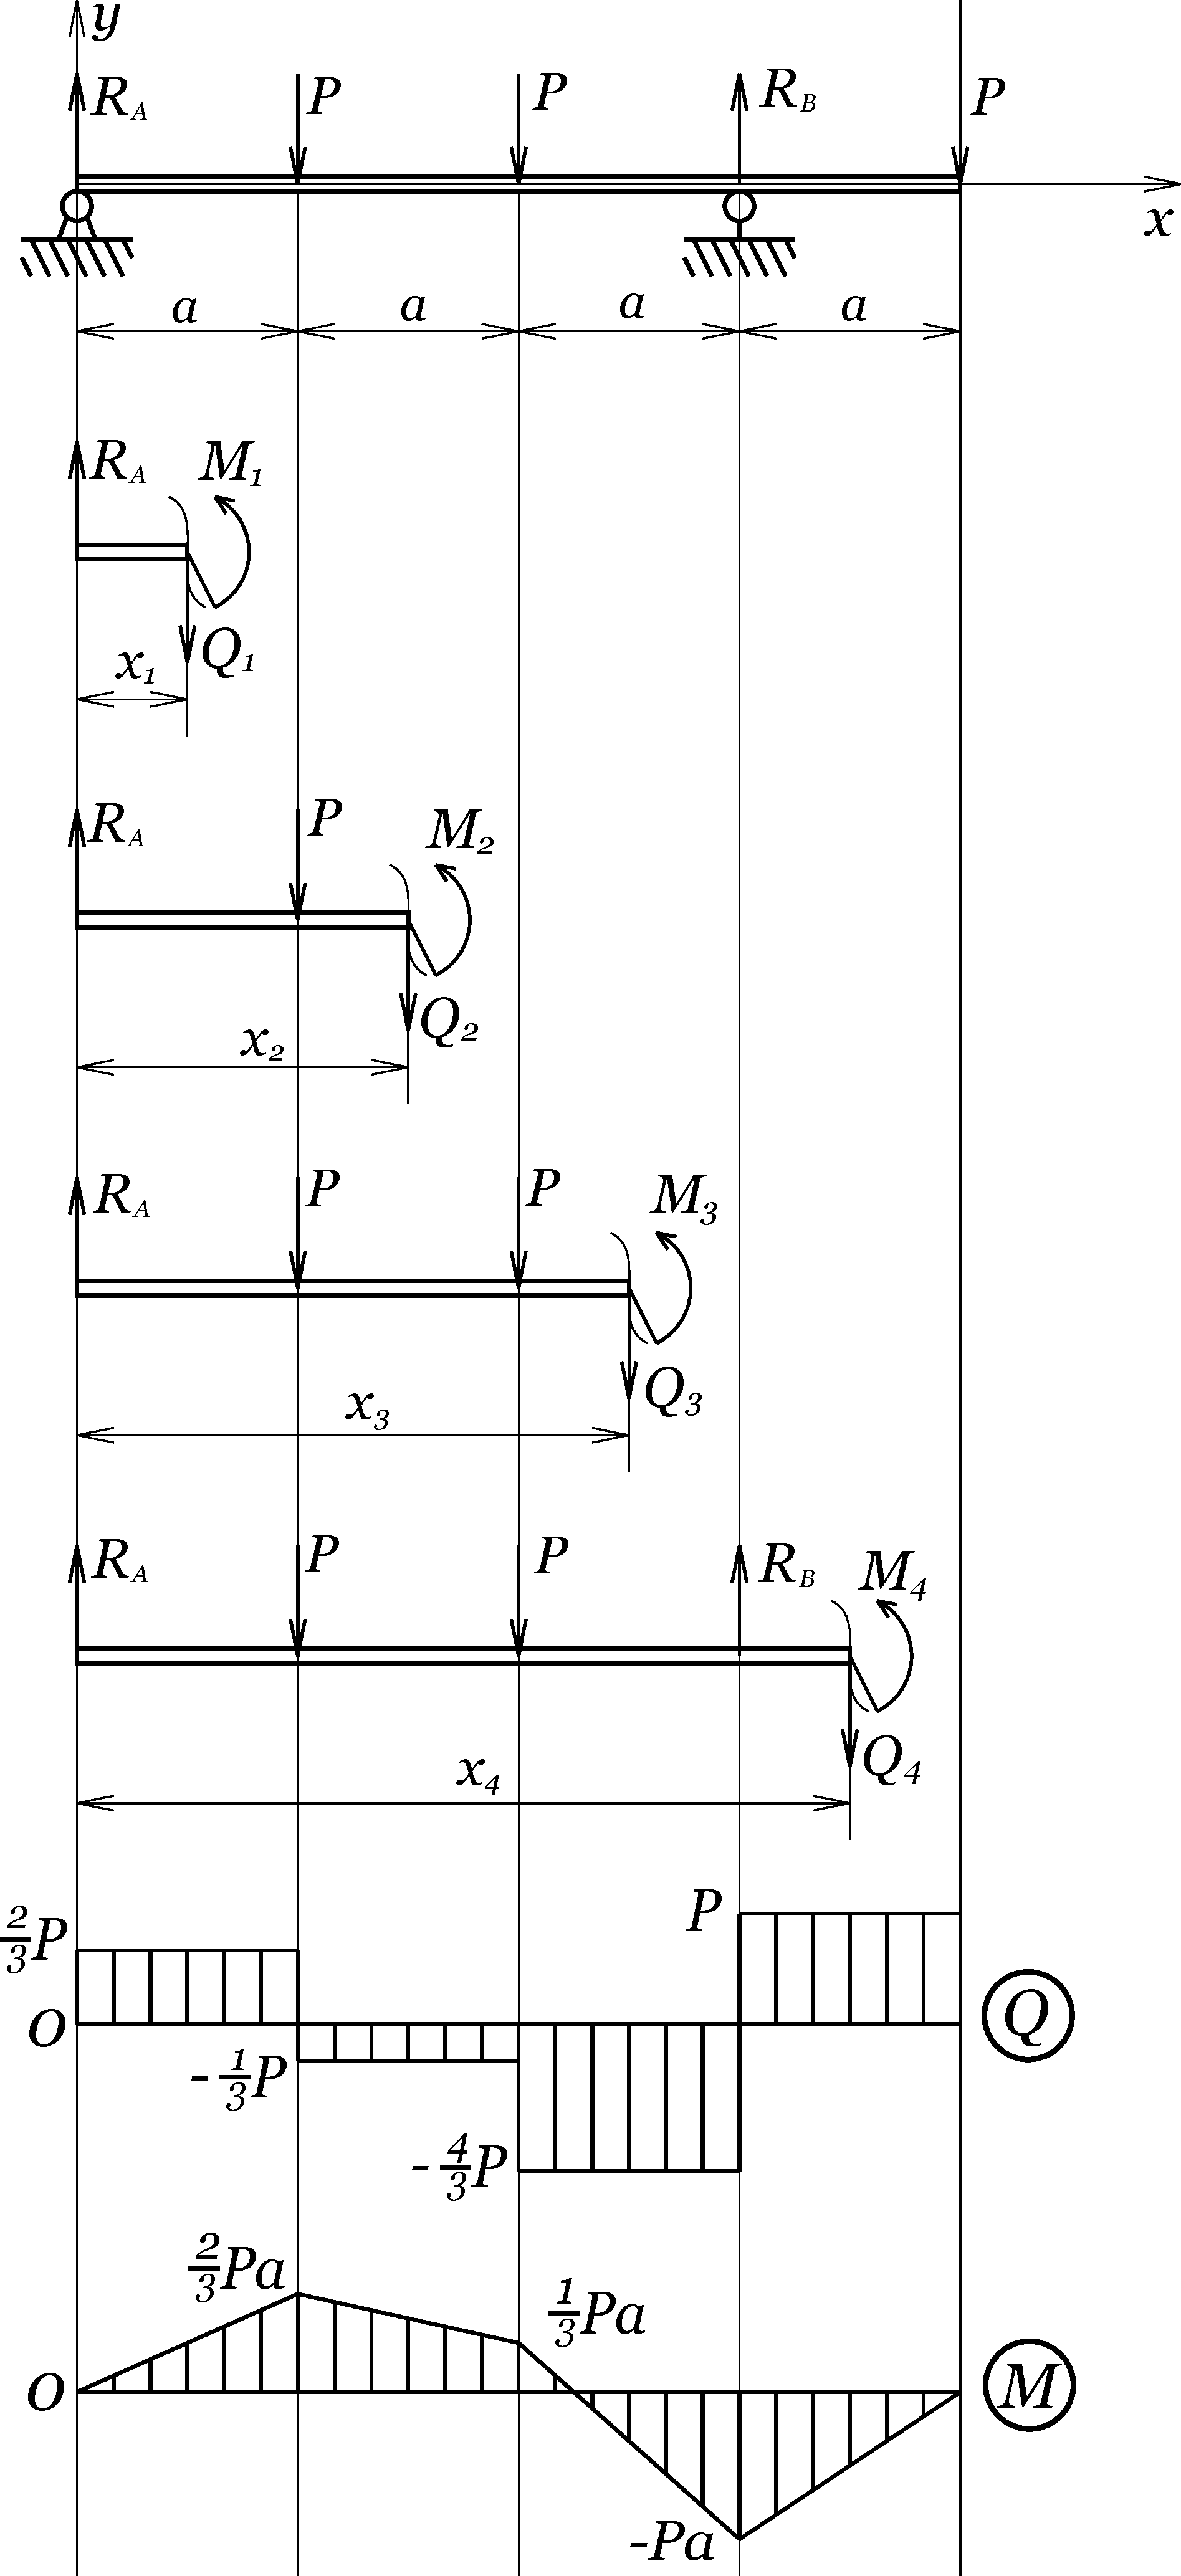
\includegraphics[width=0.5\textwidth]{epura7.pdf}
    \caption{Эпюра поперечных сил и моментов.}
    \label{fig:chap1-epura7}
\end{floatingfigure}

$\sum M_A = -Pa - 2 P a + 3 R_B a - 4 P a = 0$,
откуда
\[
    R_B = \frac{7}{3}P.
\]

$\sum M_B = 3 R_A a + 2 P a + Pa - Pa = 0$,
откуда
\[
    R_A = \frac{2}{3}P.
\]

$\sum P_y = R_A - P - P + R_B - P = 0$.

Участок 1 $\left(0 \le x < a\right)$

$\sum P_{y_1} = R_A - Q_1 = 0$,
откуда
\[
    Q_1 = \frac{2}{3}P.
\]

$\sum M_{O_1} = -R_A x + M_1 = 0$,
откуда
\[
    M_1 = \frac{2}{3} Px.
\]

При $x = 0$: $M_1 = 0$.

При $x = a$: $M_1 = \frac{2}{3} Pa$.

Участок 2 $\left(a \le x < 2a\right)$

$\sum P_{y_2} = R_A - P - Q_2 = 0$,
откуда
\[
    Q_2 = -\frac{1}{3}P.
\]

$\sum M_{O_2} = -R_A x + P (x - a) + M_2 = 0$,
откуда
\[
    M_2 = -\frac{1}{3}Px + Pa.
\]

При $x = a$: $M_2 = \frac{2}{3} Pa$.

При $x = 2 a$: $M_2 = \frac{1}{3} Pa$.

Участок 3 $\left(2a \le x < 3a\right)$

$\sum P_{y_3} = R_A - P - P - Q_3 = 0$,
откуда
\[
    Q_3 = -\frac{4}{3}P.
\]

$\sum M_{O_3} = -R_A x + P (x - a) + P (x - 2a) + M_3 = 0$,
откуда
\[
    M_3 = -\frac{4}{3}Px + 3Pa.
\]

При $x = 2 a$: $M_3 = \frac{1}{3} Pa$.

При $x = 3 a$: $M_3 = -Pa$.

Участок 4 $\left(3a \le x < 4a\right)$

$\sum P_{y_4} = R_A - P - P + R_B - Q_4 = 0$,
откуда
\[
    Q_4 = P.
\]

$\sum M_{O_4} = -R_A x + P (x - a) + P (x - 2a) - R_B (x - 3a) + M_4 = 0$,
откуда
\[
    M_4 = Px - 4Pa.
\]

При $x = 3 a$: $M_4 = -Pa$.

При $x = 4 a$: $M_4 = 0$.

\newpage


\section{Задача 8}

\begin{floatingfigure}[r]{0.5\textwidth}
    \centering
    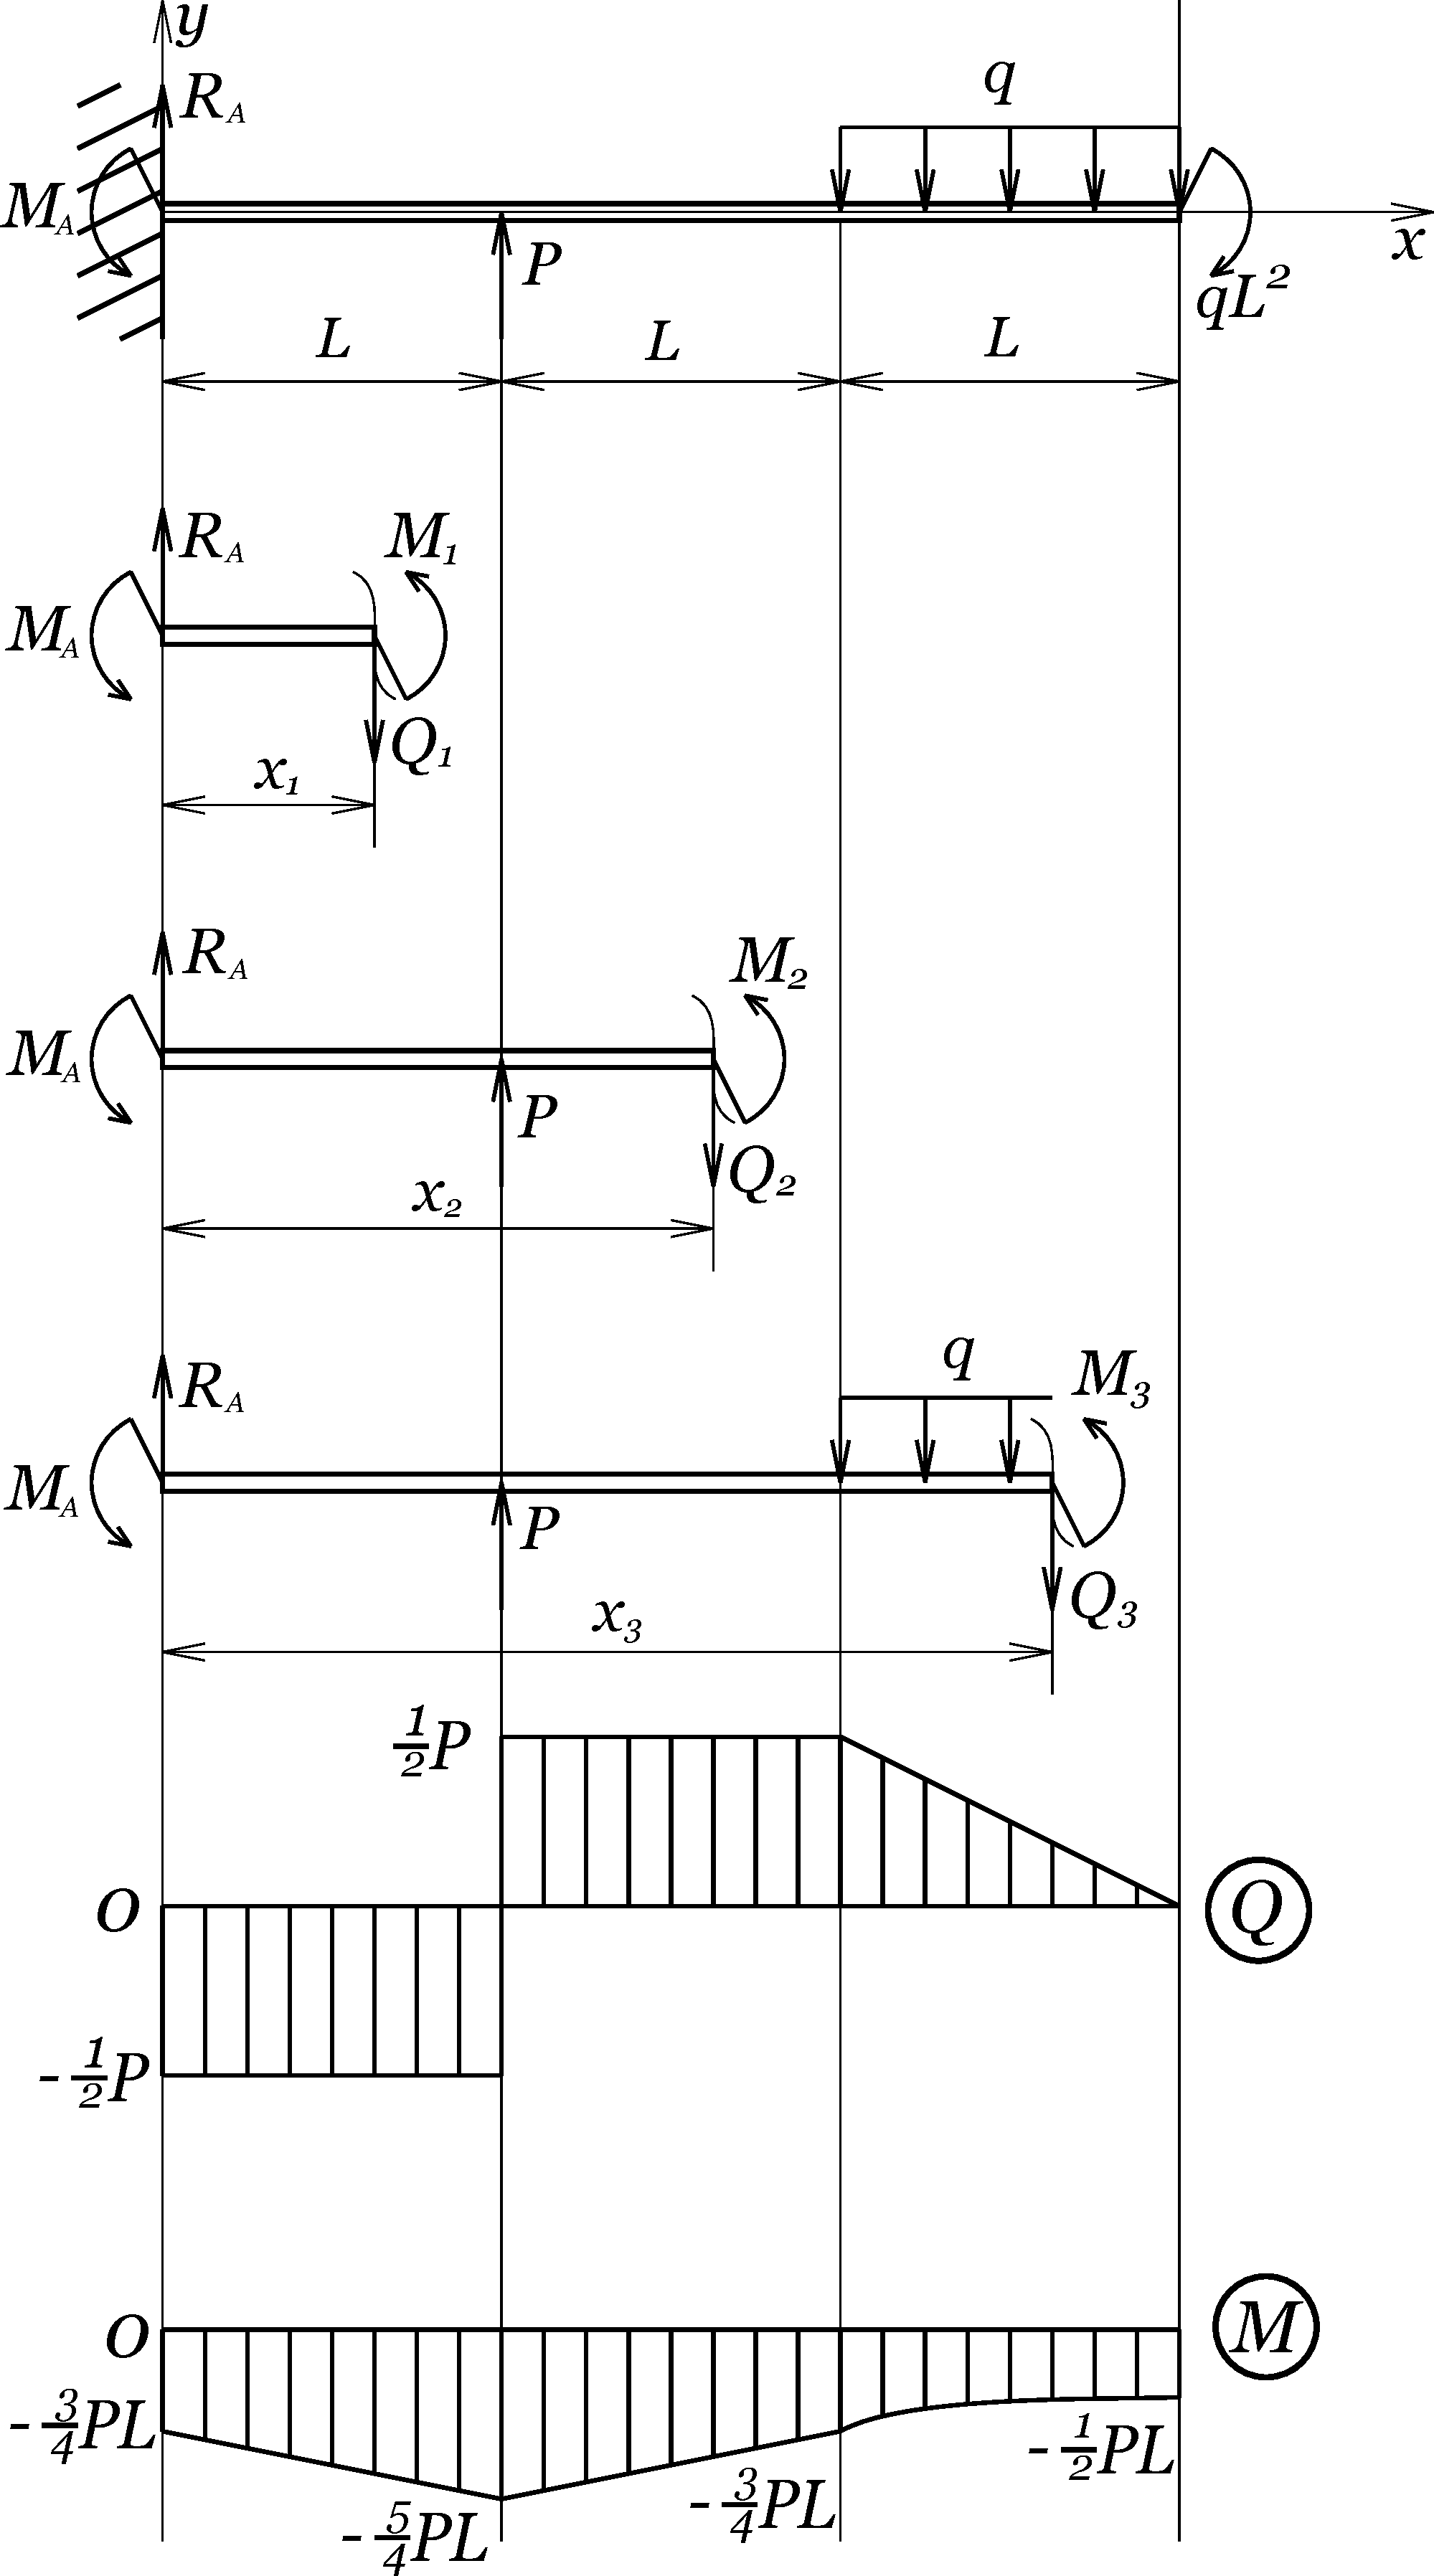
\includegraphics[width=0.5\textwidth]{epura8.pdf}
    \caption{Эпюра поперечных сил и моментов, $P = 2 q L$.}
    \label{fig:chap1-epura8}
\end{floatingfigure}

$\sum M_x = M_A + PL - q \cdot L \cdot \left(2L + \frac{L}{2}\right) - qL^2 = 0$,
откуда
\[
    M_A = \frac{3}{4}PL.
\]

$\sum P_y = -R_A - P + qL = 0$,
откуда
\[
    R_A = -\frac{1}{2}P.
\]

Участок 1 $\left(0 \le x < L\right)$

$\sum P_{y_1} = R_A - Q_1 = 0$,
откуда
\[
    Q_1 = -\frac{1}{2}P.
\]

$\sum M_{x_1} = -R_A x + M_A + M_1 = 0$,
откуда
\[
    M_1 = -\frac{1}{2}Px - \frac{3}{4}PL.
\]

При $x = 0$: $M_1 = -\frac{3}{4}PL$.

При $x = L$: $M_1 = -\frac{5}{4}PL$.

Участок 2 $\left(L \le x < 2L\right)$

$\sum P_{y_2} = R_A + P - Q_2 = 0$,
откуда
\[
    Q_2 = \frac{1}{2}P.
\]

$\sum M_{x_2} = -R_A x + M_A - P(x - L) + M_2 = 0$,
откуда
\[
    M_2 = \frac{1}{2}Px - \frac{7}{4}PL.
\]

При $x = L$: $M_2 = -\frac{5}{4}PL$.

При $x = 2L$: $M_2 = -\frac{3}{4}PL$.

Участок 3 $\left(2L \le x < 3L\right)$

$\sum P_{y_3} = R_A + P - q(x - 2L) - Q_3 = 0$,
откуда
\[
    Q_3 = -\frac{x}{2L}P + \frac{3}{2}P.
\]

При $x = 2L$: $Q_3 = \frac{1}{2}P$.

При $x = 3L$: $Q_3 = 0$.

$\sum M_{x_3} = -R_A x + M_A - P(x - L) - q(x - 2L) \cdot \frac{x-2L}{2} + M_3 = 0$,
откуда
\[
    M_3 = -\frac{1}{2}q(x - 2L)^2 + \frac{1}{2}Px - \frac{7}{4}PL.
\]

При $x = 2L$: $M_3 = -\frac{3}{4}PL$.

При $x = 3L$: $M_3 = -\frac{1}{2}PL$.

\newpage


\section{Задача 9}

\begin{floatingfigure}[r]{0.5\textwidth}
    \centering
    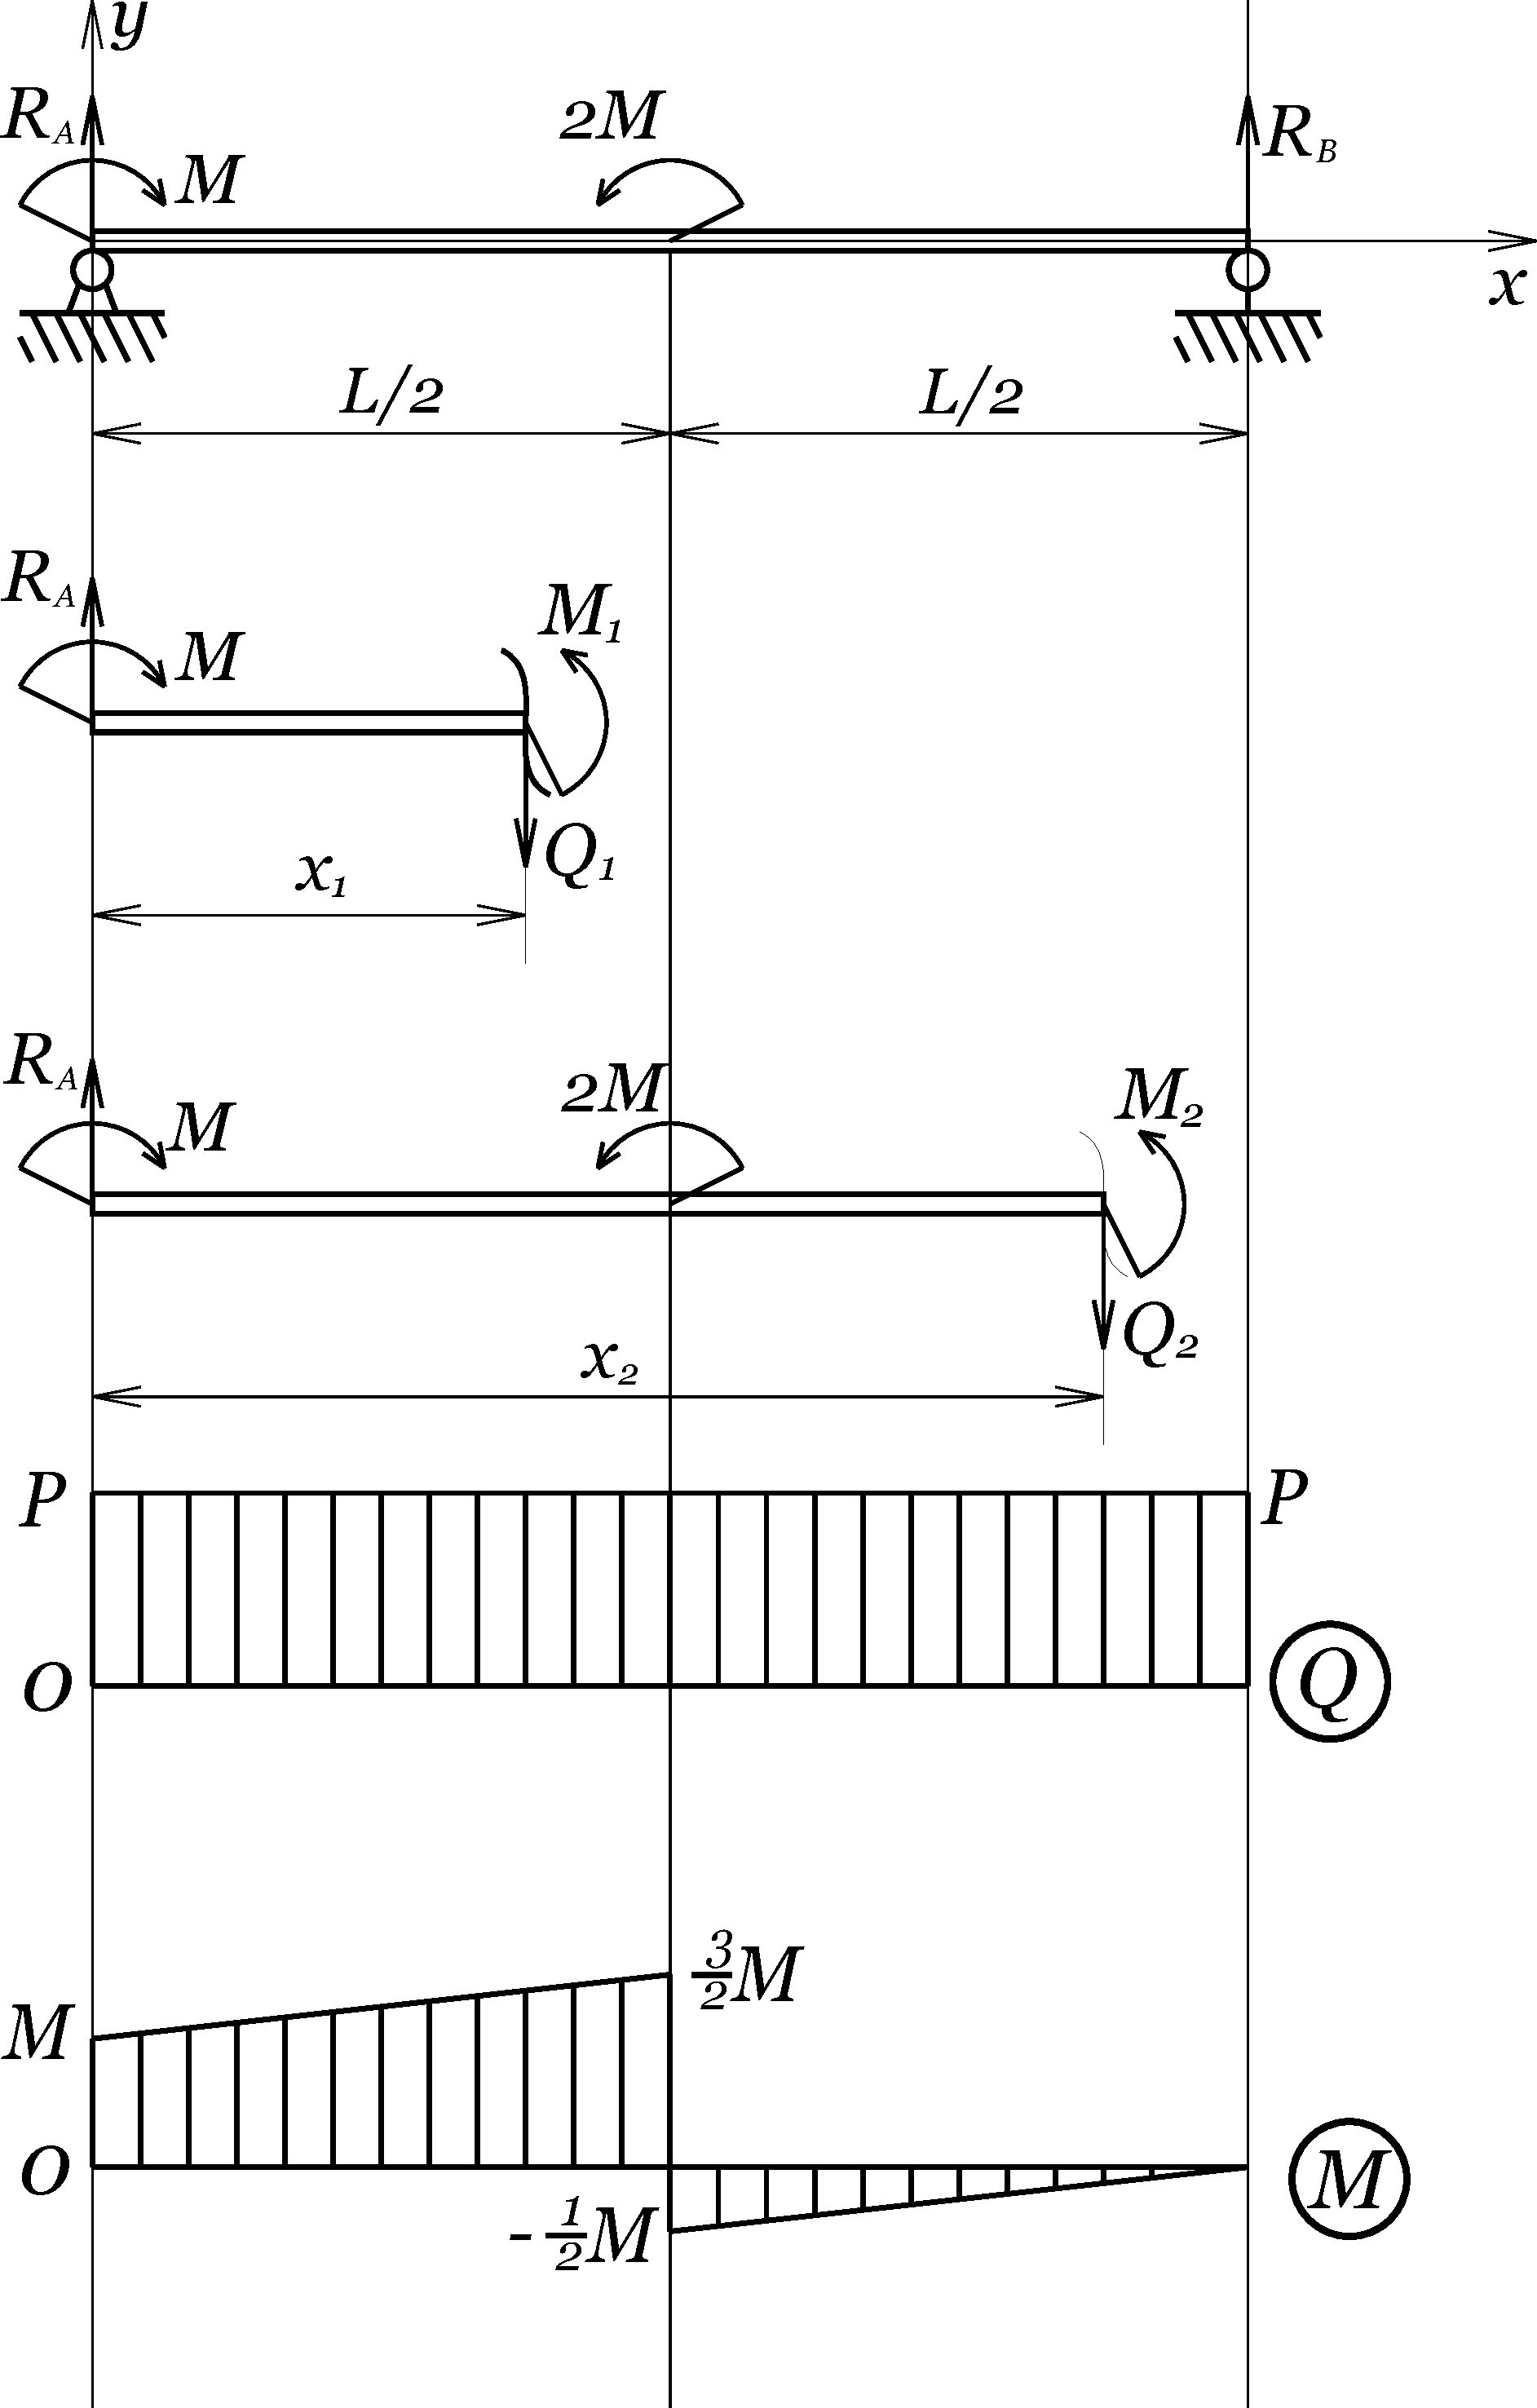
\includegraphics[width=0.5\textwidth]{epura9.pdf}
    \caption{Эпюра поперечных сил и моментов.}
    \label{fig:chap1-epura9}
\end{floatingfigure}

$\sum M_A = -M + 2M + R_B L = 0$,
откуда
\[
    R_B = -P.
\]

$\sum M_B = -R_A L - M + 2M = 0$,
откуда
\[
    R_A = P.
\]

Участок 1 $\left(0 \le x < \frac{L}{2}\right)$

$Q_{y_1} = R_A - Q_1 = 0$,
откуда
\[
    Q_1 = P.
\]

$M_{x_1} = -M - R_A x + M_1 = 0$,
откуда
\[
    M_1 = Px + M.
\]

При $x = 0$: $M_1 = M$.

При $x = \frac{L}{2}$: $M_1 = \frac{3}{2} M$.

Участок 2 $\left(\frac{L}{2} \le x < L\right)$

$Q_{y_2} = R_A - Q_2 = 0$,
откуда
\[
    Q_2 = P.
\]

$M_{x_2} = -M - R_A x + 2M + M_2 = 0$,
откуда
\[
    M_2 = Px - M.
\]

При $x = \frac{L}{2}$: $M_2 = -\frac{1}{2} M$.

При $x = L$: $M_2 = 0$.

\newpage


\section{Задача 10}

\begin{floatingfigure}[r]{0.5\textwidth}
    \centering
    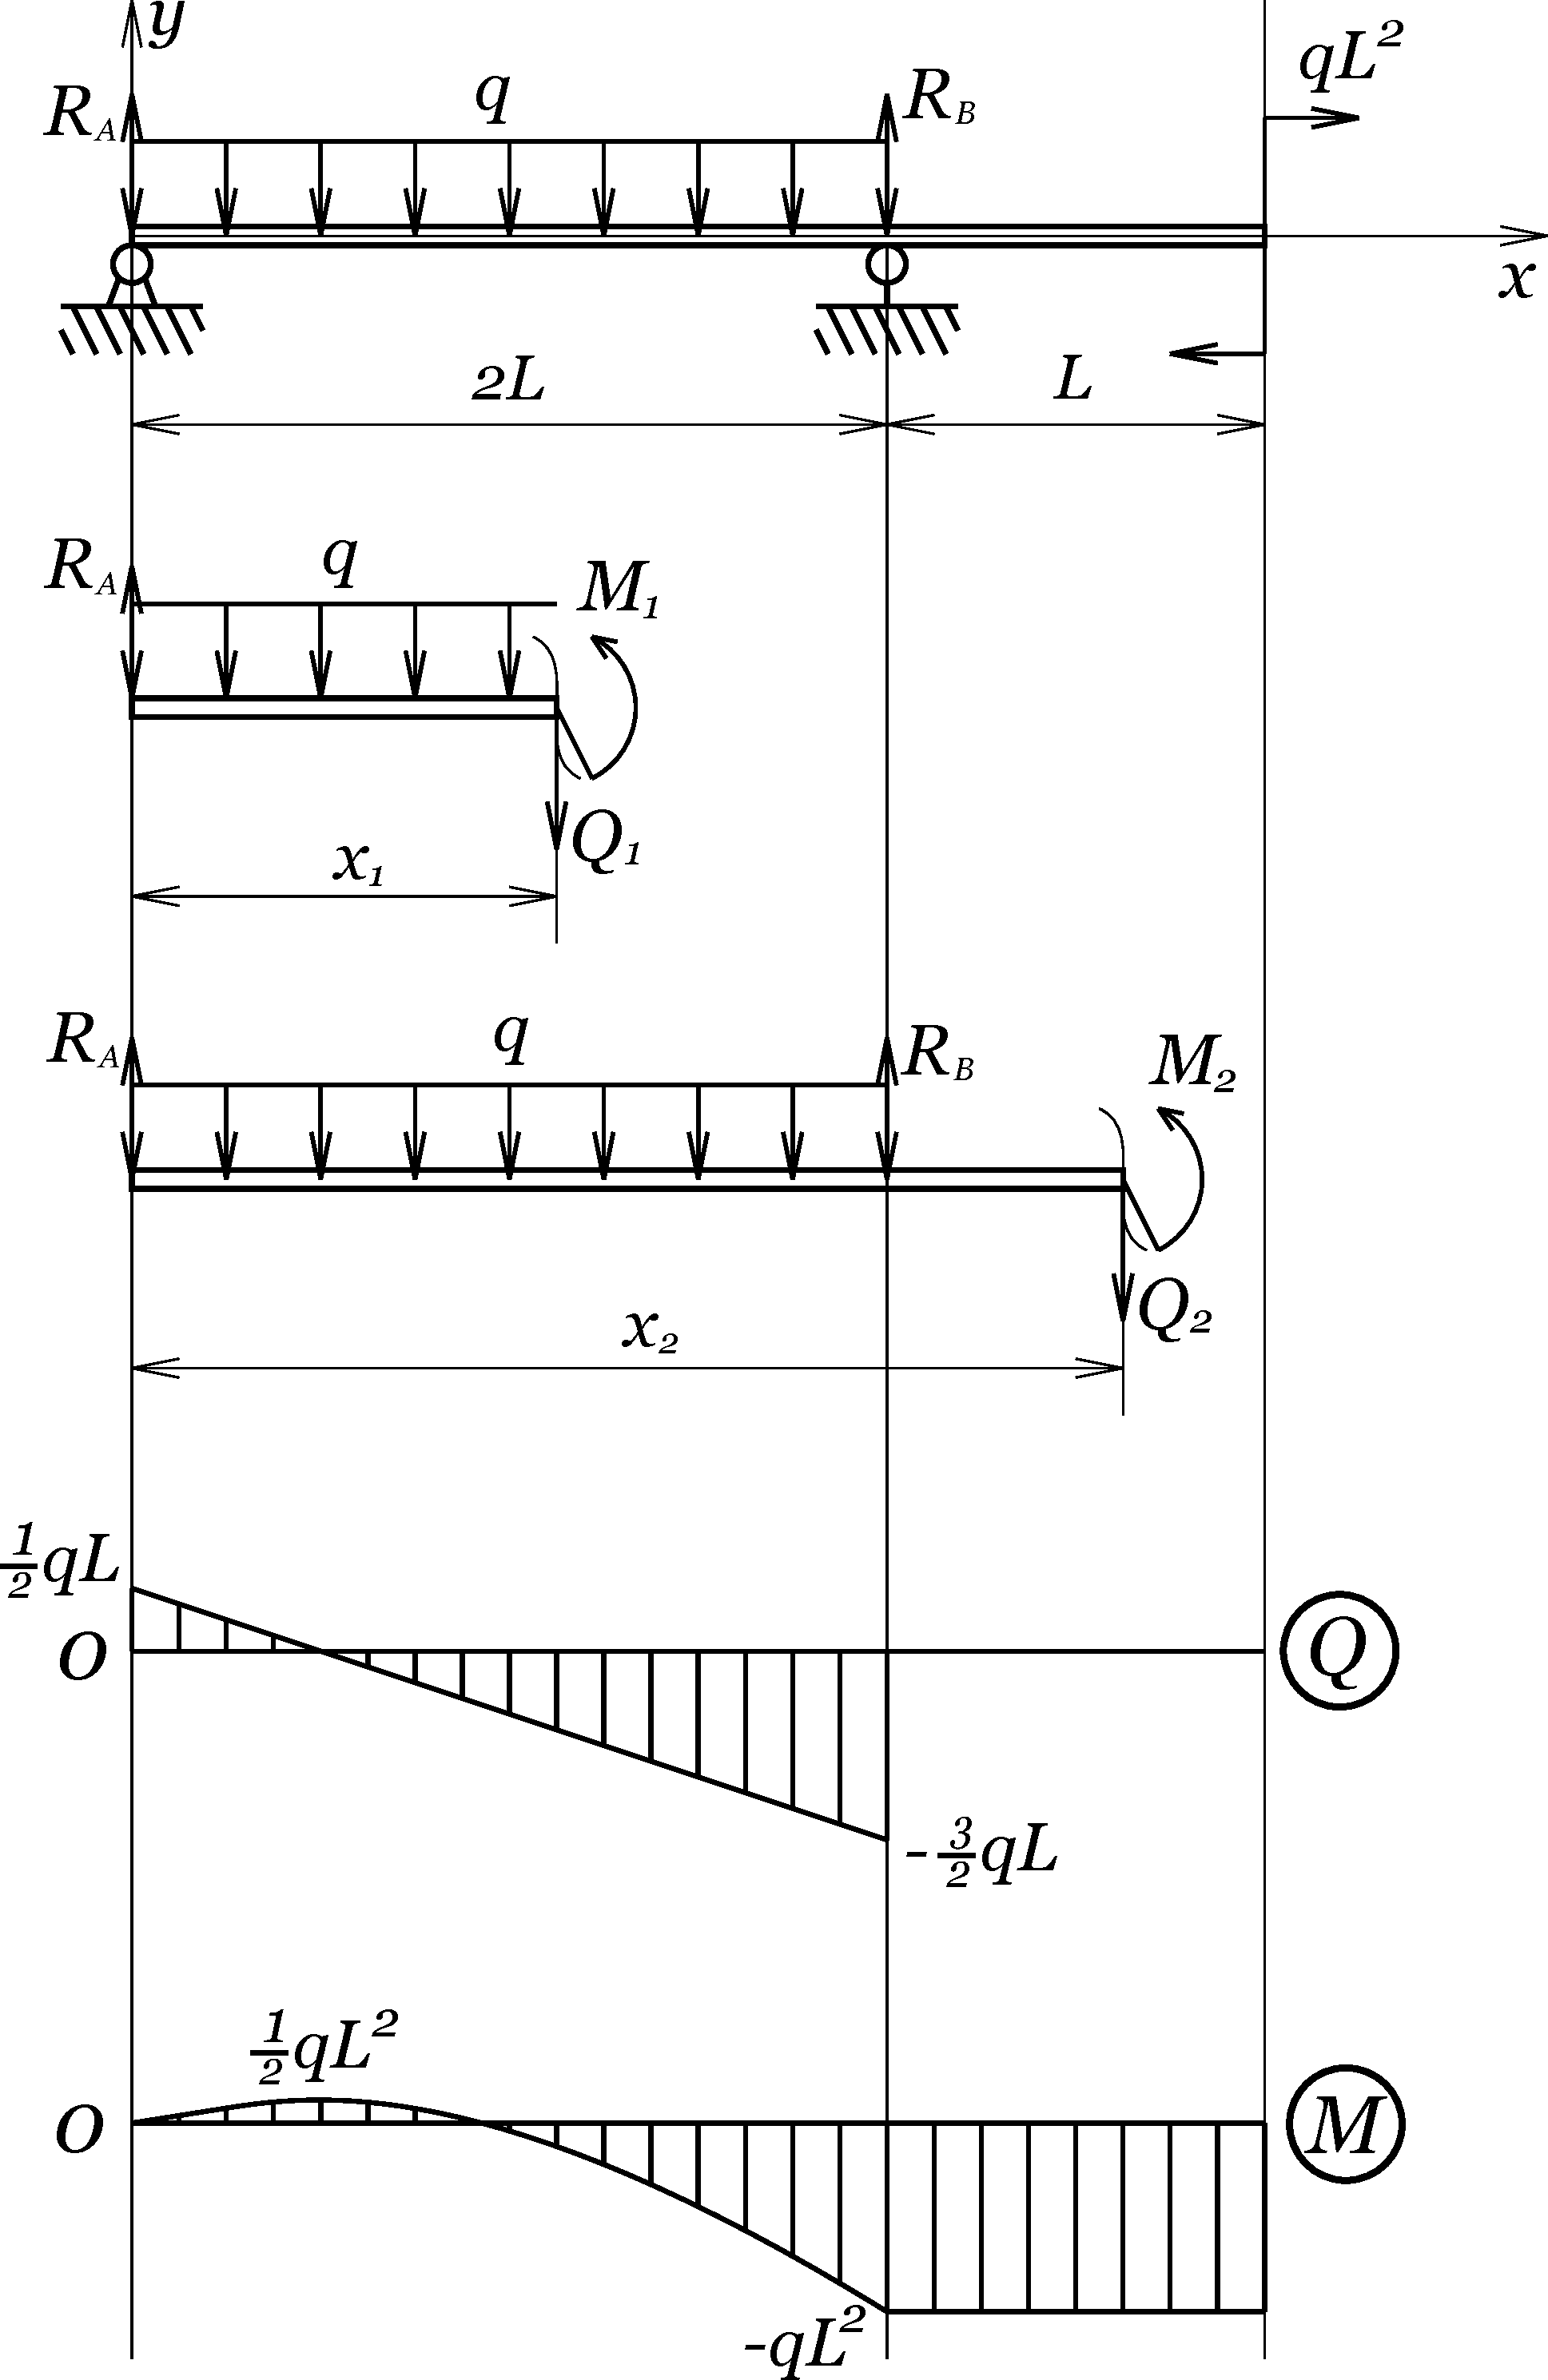
\includegraphics[width=0.5\textwidth]{epura10.pdf}
    \caption{Эпюра поперечных сил и моментов.}
    \label{fig:chap1-epura10}
\end{floatingfigure}

$\sum M_A = -q \cdot 2L \cdot L + R_B \cdot 2L - qL^2 = 0$,
откуда
\[
    R_B = \frac{3}{2}qL.
\]

$\sum M_B = -R_A \cdot 2L + q \cdot 2L \cdot L - qL^2 = 0$,
откуда
\[
    R_A = \frac{1}{2}qL.
\]

$\sum P_y = R_A - q \cdot 2L + R_B = 0$.

Участок 1 $\left(0 \le x < 2L\right)$

$\sum Q_{y_1} = R_A - qx - Q_1 = 0$,
откуда
\[
    Q_1 = -qx + \frac{1}{2}qL.
\]

При $x = 0$: $Q_1 = \frac{1}{2}qL$.

При $x = 2L$: $Q_1 = -\frac{3}{2}qL$.

$\sum M_{x_1} = -R_A x + q \cdot x \cdot \frac{1}{2}x + M_1 = 0$,
откуда
\[
    M_1 = -\frac{1}{2}qL \cdot \frac{x^2}{L} + \frac{1}{2}qLx.
\]

При $x = 0$: $M_1 = 0$.

При $x = 2L$: $M_1 = -qL^2$.

Вершина $M_1 = -qL^2$ при $x = \frac{1}{2} L$: .

Участок 2 $\left(2L \le x < 3L\right)$

$\sum Q_{y_2} = R_A - q \cdot 2L + R_B - Q_2 = 0$,
откуда
\[
    Q_2 = 0.
\]

$\sum M_{x_2} = -R_A x + q \cdot 2L \cdot (x - L) - R_B (x - 2L) + M_2 = 0$,
откуда
\[
    M_2 = -qL^2.
\]

\newpage


\section{Задача 11}

\begin{floatingfigure}[r]{0.5\textwidth}
    \centering
    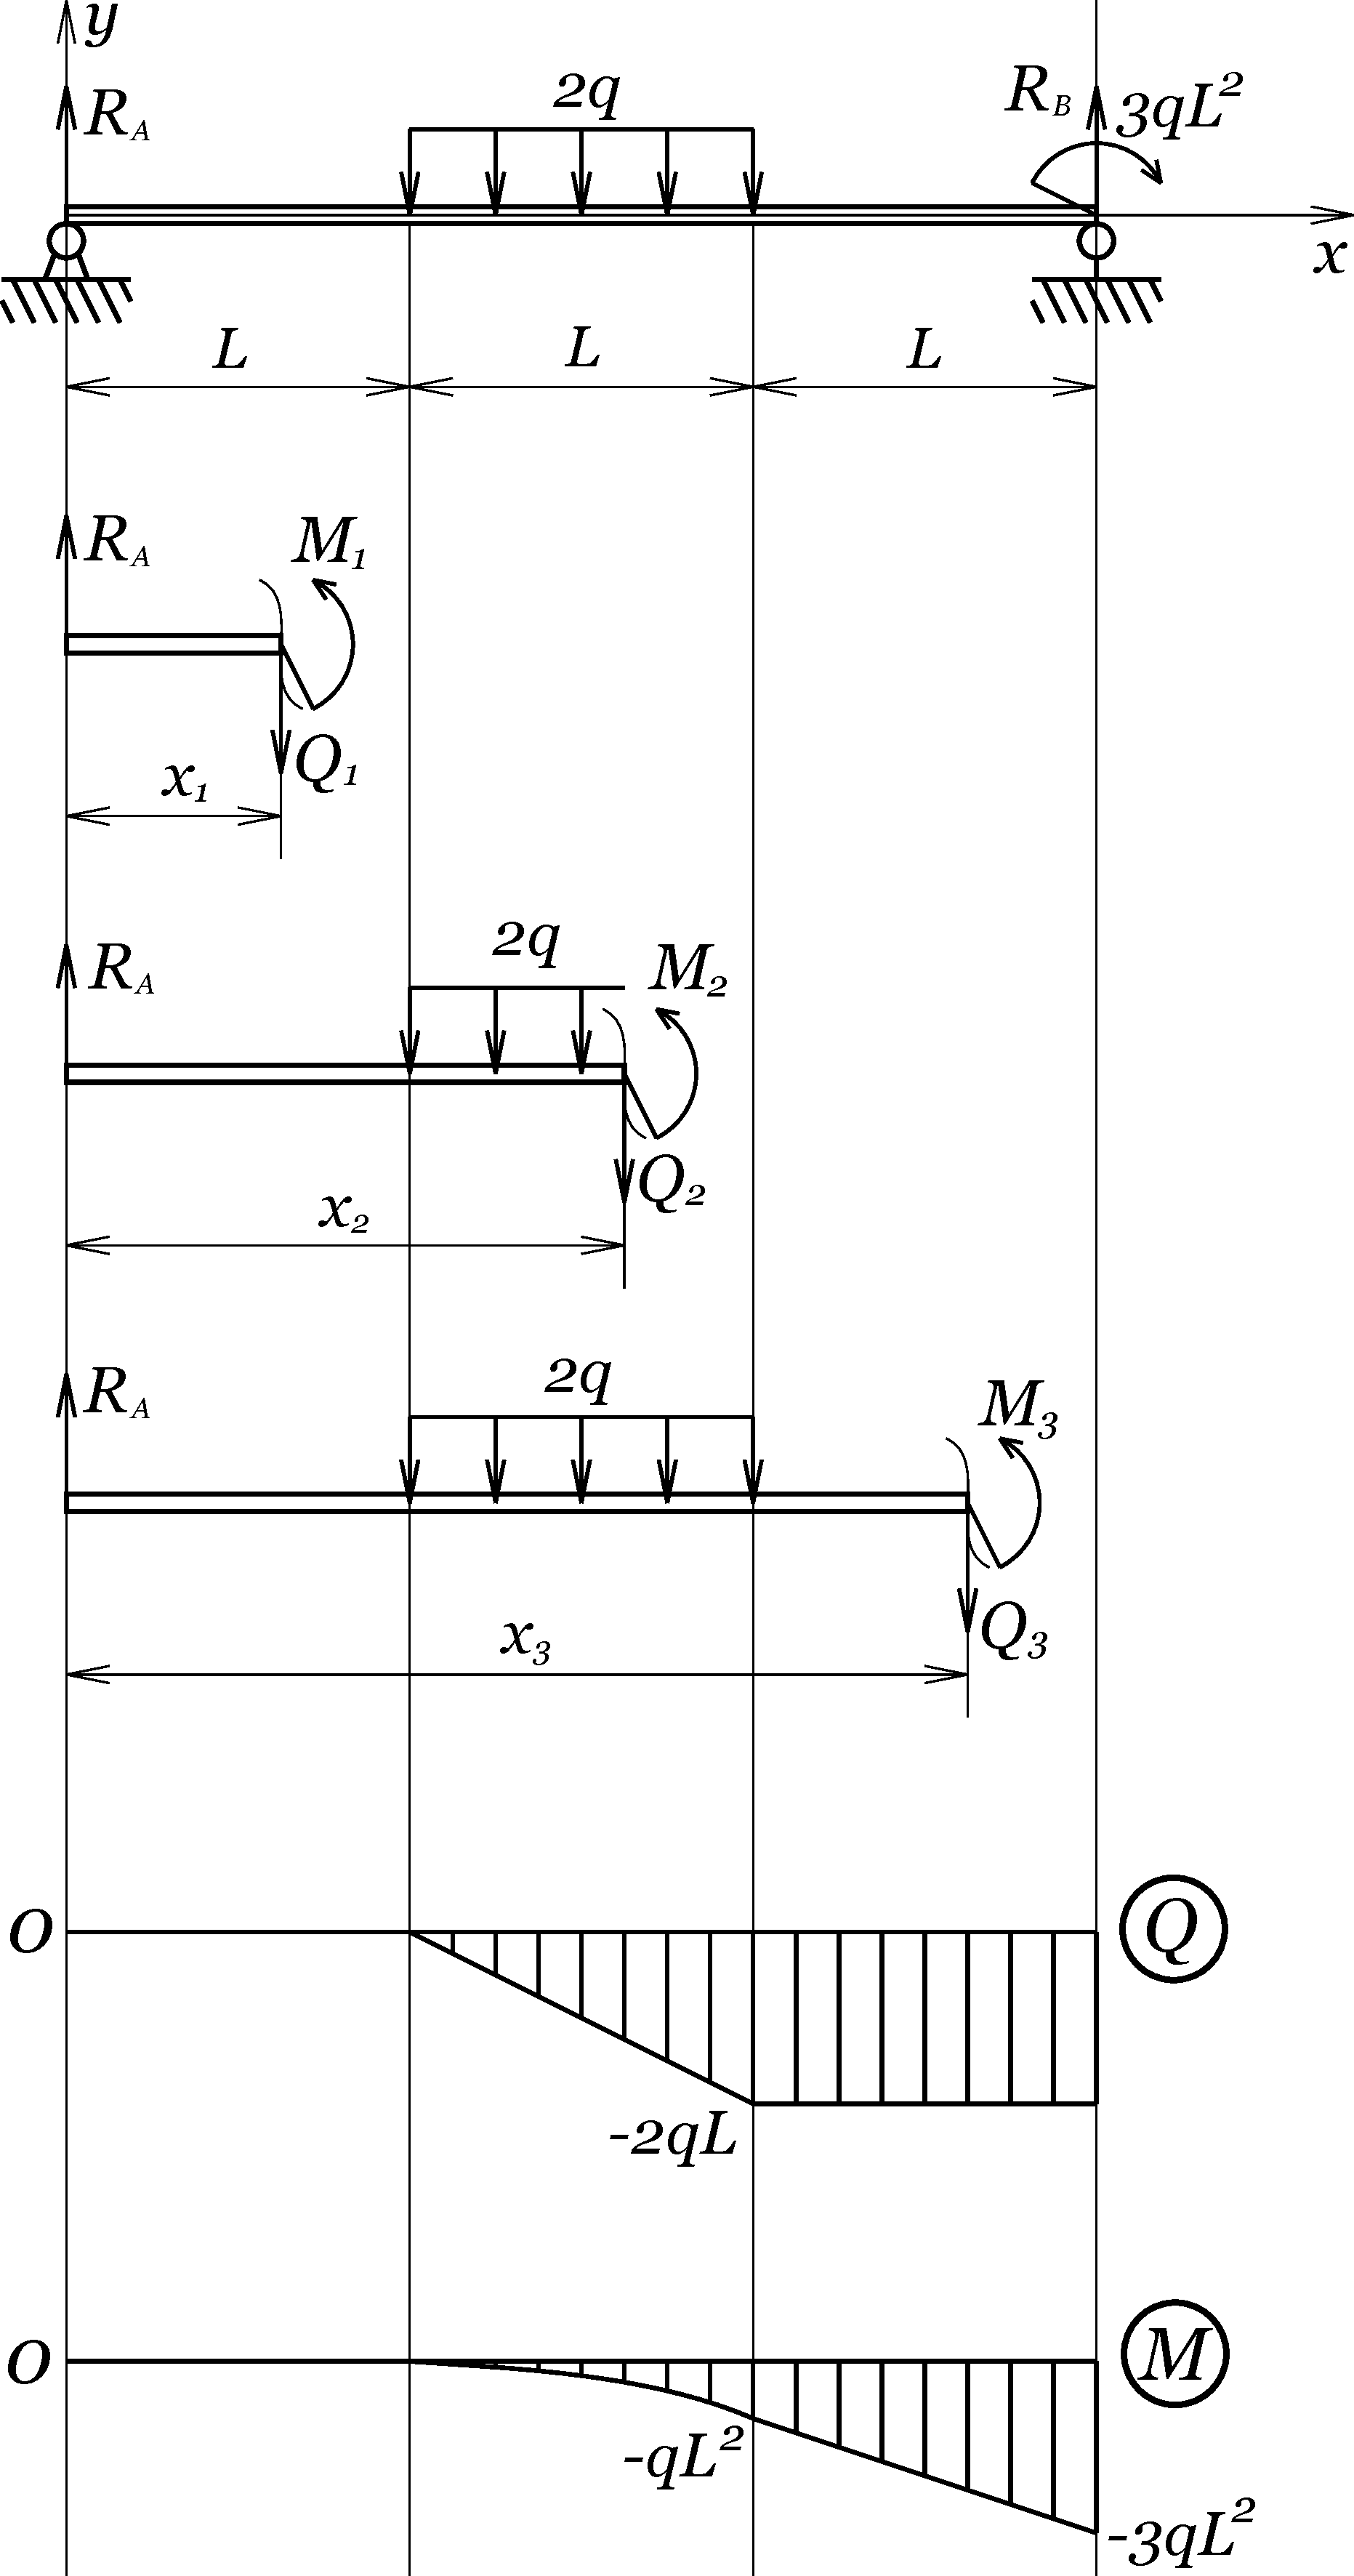
\includegraphics[width=0.5\textwidth]{epura11.pdf}
    \caption{Эпюра поперечных сил и моментов.}
    \label{fig:chap1-epura11}
\end{floatingfigure}

$\sum M_A = -2 q L \cdot \frac{3}{2} L + 3 R_B L - 3qL^2 = 0$,
откуда
\[
    R_B = 2P.
\]

$\sum M_B = -3 R_A L + 2 q L \frac{3}{2} L - 3 q L^2 = 0$,
откуда
\[
    R_A = 0.
\]

$\sum P_y = R_A - 2 q L + R_B = 0$.

Участок 1 $\left(0 \le x < L\right)$

$\sum Q_{y_1} = R_A - Q_1 = 0 $,
откуда
\[
    Q_1 = 0.
\]

$\sum M_{x_1} = -R_A x + M_1 = 0 $,
откуда
\[
    M_1 = 0.
\]

Участок 2 $\left(L \le x < 2L\right)$

$\sum Q_{y_2} = R_A - 2q(x - L) - Q_2 = 0$,
откуда
\[
    Q_2 = -2qx + 2ql.
\]

При $x = L$: $Q_2 = 0$.

При $x = 2L$: $Q_2 = -2qL$.

$\sum M_{x_2} = -R_A x + 2q (x - L) \frac{x-L}{2} + M_2 = 0$,
откуда
\[
    M_2 = -qx^2 + 2qLx - qL^2.
\]

При $x = L$: $M_2 = 0$.

При $x = 2L$: $M_2 = -qL^2$.

Участок 3 $\left(2L \le x < 3L\right)$

$\sum Q_{y_3} = R_A - 2qL - Q_3 = 0$,
откуда
\[
    Q_3 = -2qL.
\]

$\sum M_{x_3} = -R_A x + 2q L \left(x - \frac{3}{2} L\right) + M_3 = 0$,
откуда
\[
    M_3 = -2qLx + 3qL^2.
\]

При $x = 2L$: $M_3 = -qL^2$.

При $x = 3L$: $M_3 = -3qL^2$.

\newpage


\section{Задача 12}

\begin{floatingfigure}[r]{0.5\textwidth}
    \centering
    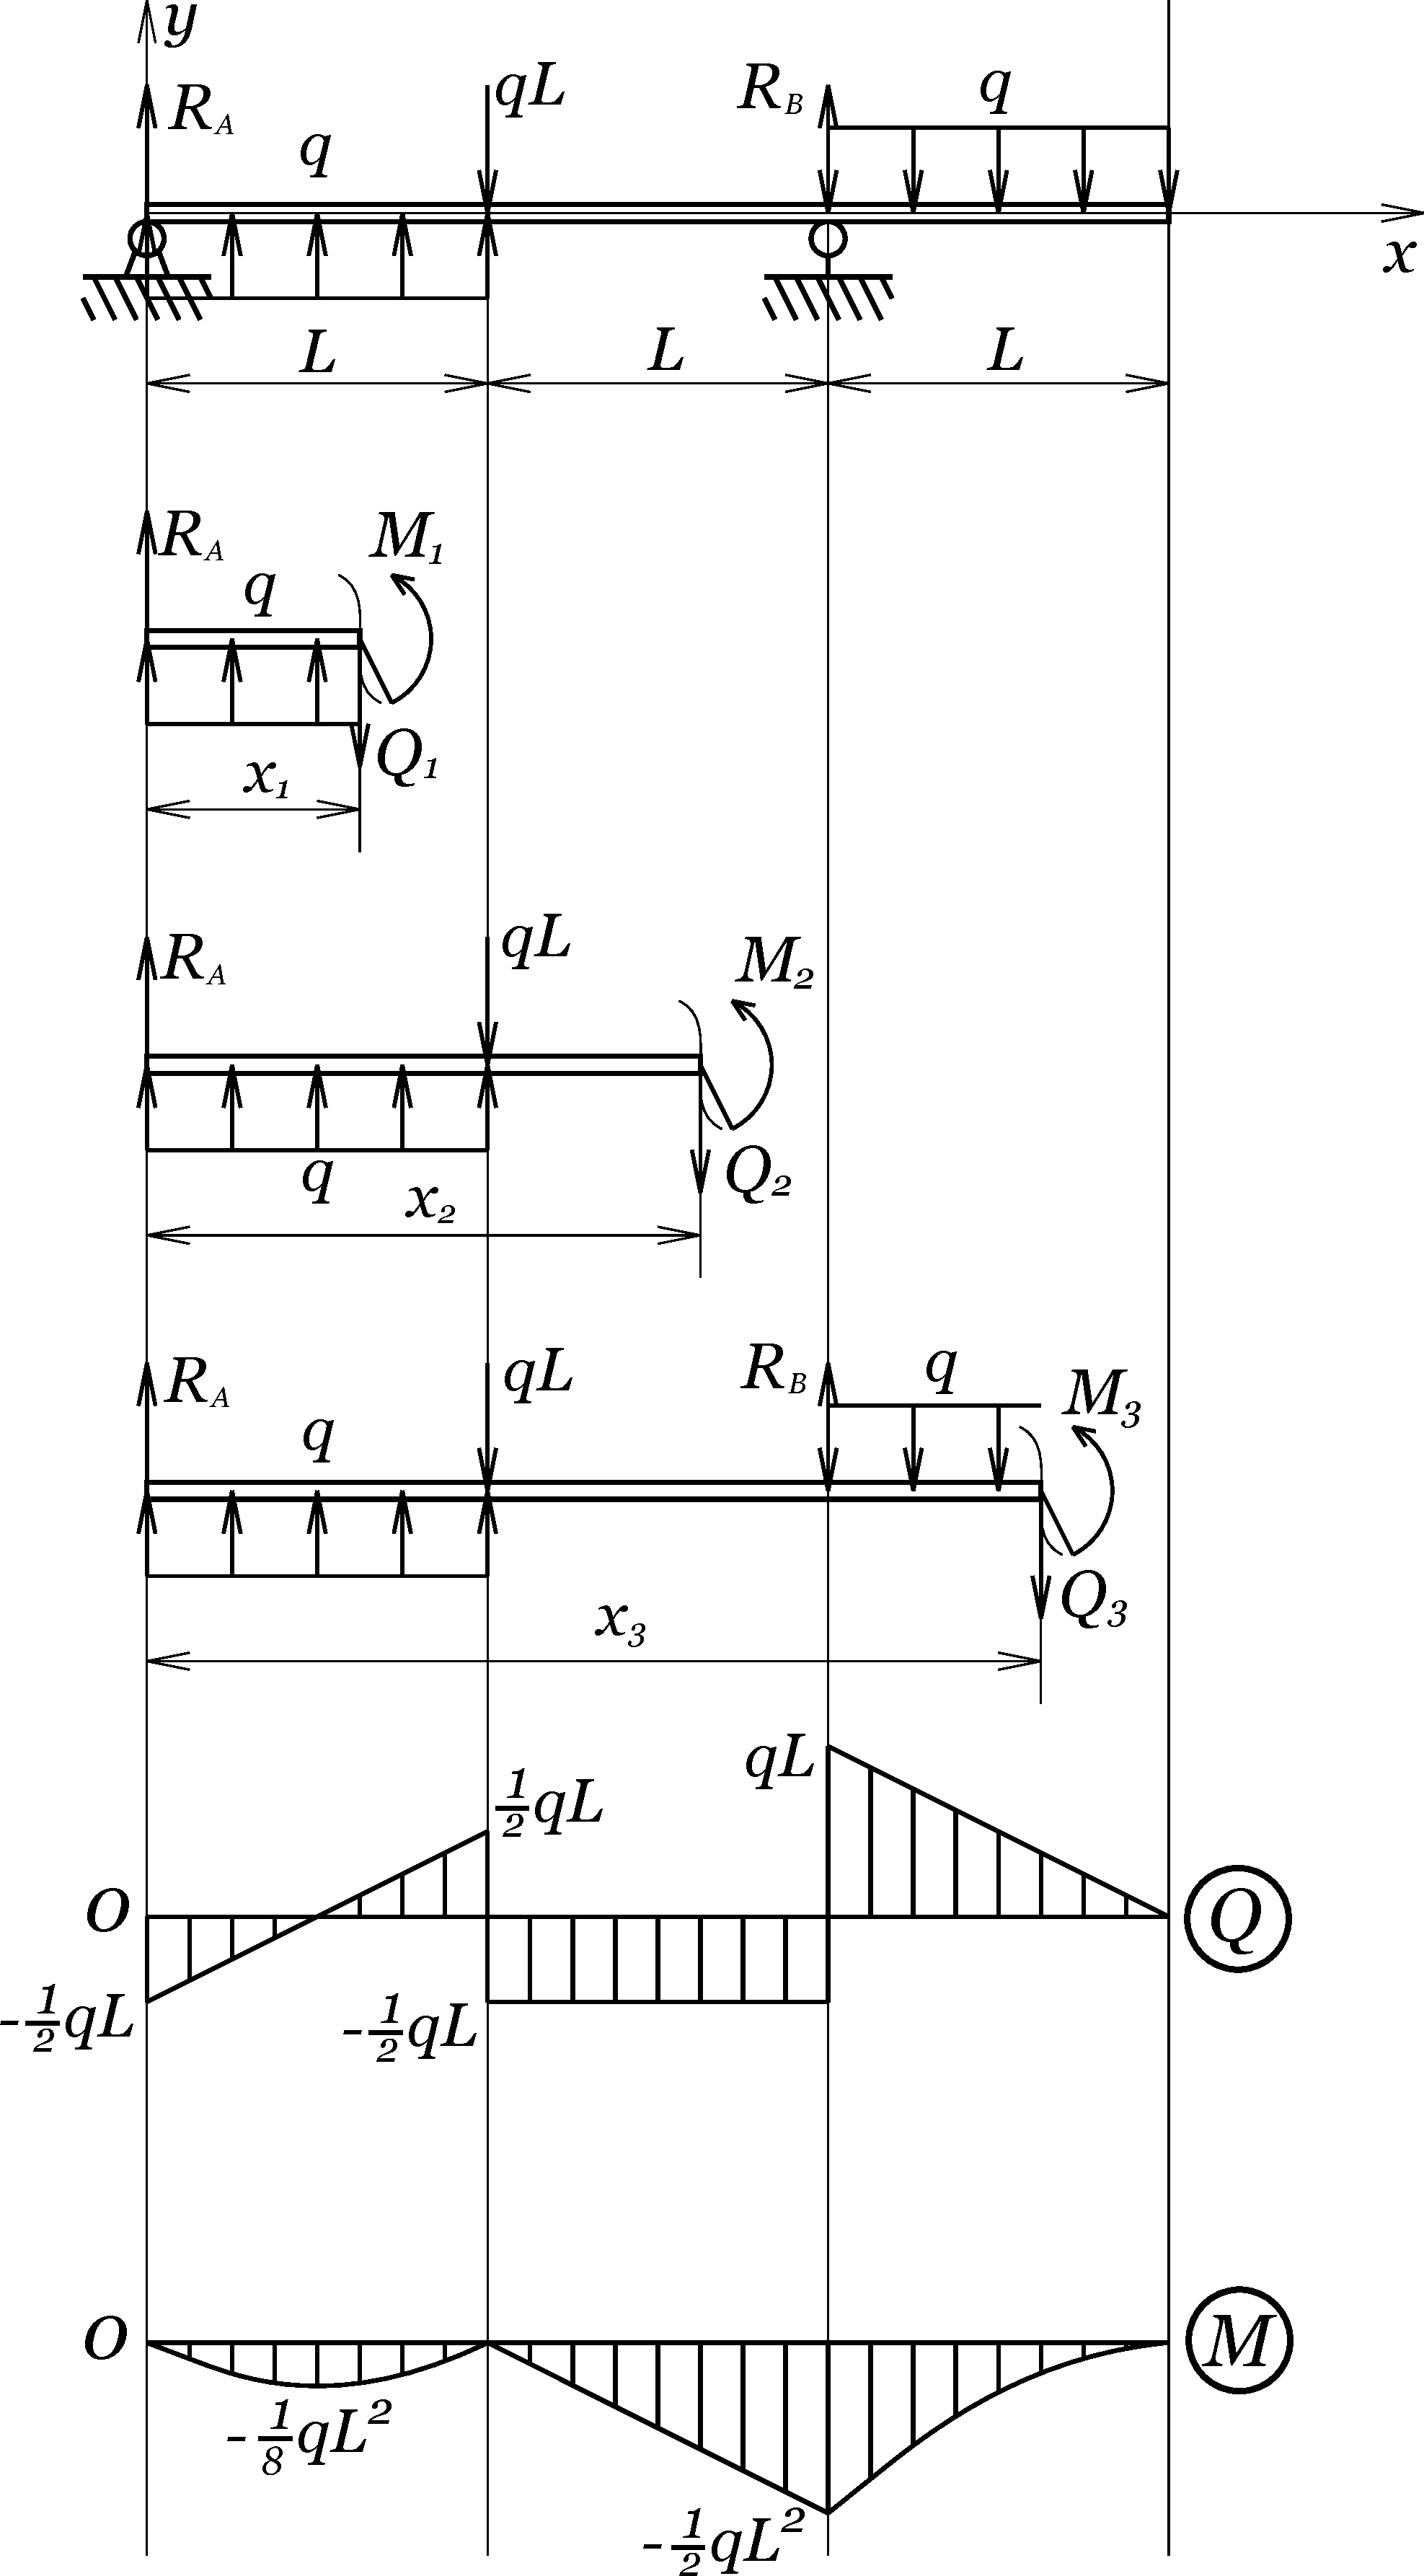
\includegraphics[width=0.5\textwidth]{epura12.pdf}
    \caption{Эпюра поперечных сил и моментов.}
    \label{fig:chap1-epura12}
\end{floatingfigure}

$\sum M_A = \frac{1}{2} q L^2 - q L^2 + 2 R_B L - \frac{5}{2} q L^2 = 0$,
откуда
\[
    R_B = \frac{3}{2} qL.
\]

$ \sum M_B = -2 R_A L - \frac{3}{2} q L^2 + q L^2 - \frac{1}{2} q L^2 = 0 $,
откуда
\[
    R_A = -\frac{1}{2} qL.
\]

$\sum P_y = R_A + qL - qL + R_B - qL = 0$

Участок 1 $\left(0 \le x < L\right)$

$\sum Q_{y_1} = R_A + qx - Q_1 = 0$,
откуда
\[
    Q_1 = qx - \frac{1}{2} qL.
\]

При $x = 0$: $Q_1 = -\frac{1}{2}qL$.

При $x = L$: $Q_1 = \frac{1}{2}qL$.

$\sum M_{x_1} = -R_A x - q \cdot x \cdot \frac{1}{2} x + M_1 = 0$,
откуда
\[
    M_1 = \frac{1}{2} qx^2 - \frac{1}{2} qL x.
\]

При $x = 0$: $M_1 = 0$.

При $x = L$: $M_1 = 0$.

Вершина $M_1 = -\frac{1}{8}qL^2$ при $x = \frac{1}{2} L$: .

Участок 2 $\left(L \le x < 2L\right)$

$\sum Q_{y_2} = R_A + qL - qL - Q_2 = 0$,
откуда
\[
    Q_2 = -\frac{1}{2} qL.
\]

$\sum M_{x_2} = -R_A x - q L (x - \frac{1}{2} L) + qL (x - L) + M_2 = 0$,
откуда
\[
    M_2 = -\frac{1}{2} qLx + \frac{1}{2} qL^2.
\]

При $x = L$: $M_2 = 0$.

При $x = 2L$: $M_2 = -\frac{1}{2}qL^2$.

Участок 3 $\left(2L \le x < 3L\right)$

$\sum Q_{y_3} = R_A + qL - qL - q(x - 2L) - Q_3 = 0$,
откуда
\[
    Q_3 = -qx + 3qL.
\]

При $x = 2L$: $Q_3 = qL$.

При $x = 3L$: $Q_3 = 0$.

$\sum M_{x_3} = -R_A x - q L (x - \frac{1}{2} L) + qL (x - L) - R_B (x - 2L) + q (x - 2L) \frac{x-2L}{2} + M_3 = 0$,
откуда 
\[
    M_3 = -\frac{1}{2} qx^2 + 3qLx - \frac{9}{2} qL^2.
\]

При $x = 2L$: $M_3 = -\frac{1}{2}qL^2$.

При $x = 3L$: $M_3 = 0$.

